\documentclass[twoside]{book}

% Packages required by doxygen
\usepackage{calc}
\usepackage{doxygen}
\usepackage{graphicx}
\usepackage[utf8]{inputenc}
\usepackage{makeidx}
\usepackage{multicol}
\usepackage{multirow}
\usepackage{textcomp}
\usepackage[table]{xcolor}

% Font selection
\usepackage[T1]{fontenc}
\usepackage{mathptmx}
\usepackage[scaled=.90]{helvet}
\usepackage{courier}
\usepackage{amssymb}
\usepackage{sectsty}
\renewcommand{\familydefault}{\sfdefault}
\allsectionsfont{%
  \fontseries{bc}\selectfont%
  \color{darkgray}%
}
\renewcommand{\DoxyLabelFont}{%
  \fontseries{bc}\selectfont%
  \color{darkgray}%
}

% Page & text layout
\usepackage{geometry}
\geometry{%
  a4paper,%
  top=2.5cm,%
  bottom=2.5cm,%
  left=2.5cm,%
  right=2.5cm%
}
\tolerance=750
\hfuzz=15pt
\hbadness=750
\setlength{\emergencystretch}{15pt}
\setlength{\parindent}{0cm}
\setlength{\parskip}{0.2cm}
\makeatletter
\renewcommand{\paragraph}{%
  \@startsection{paragraph}{4}{0ex}{-1.0ex}{1.0ex}{%
    \normalfont\normalsize\bfseries\SS@parafont%
  }%
}
\renewcommand{\subparagraph}{%
  \@startsection{subparagraph}{5}{0ex}{-1.0ex}{1.0ex}{%
    \normalfont\normalsize\bfseries\SS@subparafont%
  }%
}
\makeatother

% Headers & footers
\usepackage{fancyhdr}
\pagestyle{fancyplain}
\fancyhead[LE]{\fancyplain{}{\bfseries\thepage}}
\fancyhead[CE]{\fancyplain{}{}}
\fancyhead[RE]{\fancyplain{}{\bfseries\leftmark}}
\fancyhead[LO]{\fancyplain{}{\bfseries\rightmark}}
\fancyhead[CO]{\fancyplain{}{}}
\fancyhead[RO]{\fancyplain{}{\bfseries\thepage}}
\fancyfoot[LE]{\fancyplain{}{}}
\fancyfoot[CE]{\fancyplain{}{}}
\fancyfoot[RE]{\fancyplain{}{\bfseries\scriptsize Generated on Mon Sep 15 2014 23\-:40\-:21 for S\-I\-M\-P\-L\-E C\-L\-U\-S\-T\-E\-R\-S by Doxygen }}
\fancyfoot[LO]{\fancyplain{}{\bfseries\scriptsize Generated on Mon Sep 15 2014 23\-:40\-:21 for S\-I\-M\-P\-L\-E C\-L\-U\-S\-T\-E\-R\-S by Doxygen }}
\fancyfoot[CO]{\fancyplain{}{}}
\fancyfoot[RO]{\fancyplain{}{}}
\renewcommand{\footrulewidth}{0.4pt}
\renewcommand{\chaptermark}[1]{%
  \markboth{#1}{}%
}
\renewcommand{\sectionmark}[1]{%
  \markright{\thesection\ #1}%
}

% Indices & bibliography
\usepackage{natbib}
\usepackage[titles]{tocloft}
\setcounter{tocdepth}{3}
\setcounter{secnumdepth}{5}
\makeindex

% Hyperlinks (required, but should be loaded last)
\usepackage{ifpdf}
\ifpdf
  \usepackage[pdftex,pagebackref=true]{hyperref}
\else
  \usepackage[ps2pdf,pagebackref=true]{hyperref}
\fi
\hypersetup{%
  colorlinks=true,%
  linkcolor=blue,%
  citecolor=blue,%
  unicode%
}

% Custom commands
\newcommand{\clearemptydoublepage}{%
  \newpage{\pagestyle{empty}\cleardoublepage}%
}


%===== C O N T E N T S =====

\begin{document}

% Titlepage & ToC
\hypersetup{pageanchor=false}
\pagenumbering{roman}
\begin{titlepage}
\vspace*{7cm}
\begin{center}%
{\Large S\-I\-M\-P\-L\-E C\-L\-U\-S\-T\-E\-R\-S \\[1ex]\large 1.\-0 }\\
\vspace*{1cm}
{\large Generated by Doxygen 1.8.6}\\
\vspace*{0.5cm}
{\small Mon Sep 15 2014 23:40:21}\\
\end{center}
\end{titlepage}
\clearemptydoublepage
\tableofcontents
\clearemptydoublepage
\pagenumbering{arabic}
\hypersetup{pageanchor=true}

%--- Begin generated contents ---
\chapter{Namespace Index}
\section{Namespace List}
Here is a list of all documented namespaces with brief descriptions\-:\begin{DoxyCompactList}
\item\contentsline{section}{\hyperlink{namespaceSimpleCluster}{Simple\-Cluster} }{\pageref{namespaceSimpleCluster}}{}
\end{DoxyCompactList}

\chapter{Hierarchical Index}
\section{Class Hierarchy}
This inheritance list is sorted roughly, but not completely, alphabetically\-:\begin{DoxyCompactList}
\item \contentsline{section}{Simple\-Cluster\-:\-:K\-D\-Node$<$ Data\-Type $>$}{\pageref{classSimpleCluster_1_1KDNode}}{}
\item \contentsline{section}{Simple\-Cluster\-:\-:Kmeans\-Criteria}{\pageref{structSimpleCluster_1_1KmeansCriteria}}{}
\item Test\begin{DoxyCompactList}
\item \contentsline{section}{K\-D\-Tree\-Test}{\pageref{classKDTreeTest}}{}
\item \contentsline{section}{Kmeans\-Test}{\pageref{classKmeansTest}}{}
\item \contentsline{section}{Util\-Test}{\pageref{classUtilTest}}{}
\end{DoxyCompactList}
\end{DoxyCompactList}

\chapter{Class Index}
\section{Class List}
Here are the classes, structs, unions and interfaces with brief descriptions\+:\begin{DoxyCompactList}
\item\contentsline{section}{\hyperlink{classSimpleCluster_1_1KDNode}{Simple\+Cluster\+::\+K\+D\+Node$<$ Data\+Type $>$} }{\pageref{classSimpleCluster_1_1KDNode}}{}
\item\contentsline{section}{\hyperlink{classKDTreeTest}{K\+D\+Tree\+Test} }{\pageref{classKDTreeTest}}{}
\item\contentsline{section}{\hyperlink{structSimpleCluster_1_1KmeansCriteria}{Simple\+Cluster\+::\+Kmeans\+Criteria} }{\pageref{structSimpleCluster_1_1KmeansCriteria}}{}
\item\contentsline{section}{\hyperlink{classKmeansTest}{Kmeans\+Test} }{\pageref{classKmeansTest}}{}
\item\contentsline{section}{\hyperlink{classUtilTest}{Util\+Test} }{\pageref{classUtilTest}}{}
\end{DoxyCompactList}

\chapter{Namespace Documentation}
\hypertarget{namespaceSimpleCluster}{\section{Simple\+Cluster Namespace Reference}
\label{namespaceSimpleCluster}\index{Simple\+Cluster@{Simple\+Cluster}}
}
\subsection*{Classes}
\begin{DoxyCompactItemize}
\item 
class \hyperlink{classSimpleCluster_1_1KDNode}{K\+D\+Node}
\item 
struct \hyperlink{structSimpleCluster_1_1KmeansCriteria}{Kmeans\+Criteria}
\end{DoxyCompactItemize}
\subsection*{Typedefs}
\begin{DoxyCompactItemize}
\item 
\hypertarget{namespaceSimpleCluster_a2c39f662ef8ab290b2a0613dbc3b4c4e}{typedef vector$<$ double $>$ {\bfseries d\+\_\+vector}}\label{namespaceSimpleCluster_a2c39f662ef8ab290b2a0613dbc3b4c4e}

\item 
\hypertarget{namespaceSimpleCluster_ab17abba17860f283d1defd90861cb798}{typedef vector$<$ int $>$ {\bfseries i\+\_\+vector}}\label{namespaceSimpleCluster_ab17abba17860f283d1defd90861cb798}

\end{DoxyCompactItemize}
\subsection*{Enumerations}
\begin{DoxyCompactItemize}
\item 
enum \hyperlink{namespaceSimpleCluster_a1ad2d6129171ff9a5ee57f48b5f3f6e1}{Kmeans\+Assign\+Type} \{ {\bfseries L\+I\+N\+E\+A\+R}, 
{\bfseries N\+N\+\_\+\+K\+D\+\_\+\+T\+R\+E\+E}, 
{\bfseries A\+N\+N\+\_\+\+K\+D\+\_\+\+T\+R\+E\+E}
 \}
\item 
enum \hyperlink{namespaceSimpleCluster_a8a8f57121b69a7b43575e4d6a53928e2}{Kmeans\+Type} \{ {\bfseries R\+A\+N\+D\+O\+M\+\_\+\+S\+E\+E\+D\+S}, 
{\bfseries K\+M\+E\+A\+N\+S\+\_\+\+P\+L\+U\+S\+\_\+\+S\+E\+E\+D\+S}, 
{\bfseries U\+S\+E\+R\+\_\+\+S\+E\+E\+D\+S}
 \}
\end{DoxyCompactItemize}
\subsection*{Functions}
\begin{DoxyCompactItemize}
\item 
void \hyperlink{namespaceSimpleCluster_aa3c1fa27364305d35f14eb0b6b984a10}{random\+\_\+seeds} (size\+\_\+t, size\+\_\+t, size\+\_\+t, double $\ast$$\ast$, double $\ast$$\ast$\&, bool)
\item 
void \hyperlink{namespaceSimpleCluster_ab1abfee692e0476f34c72ac18a68bf17}{kmeans\+\_\+pp\+\_\+seeds} (size\+\_\+t, size\+\_\+t, size\+\_\+t, double $\ast$$\ast$, double $\ast$$\ast$\&, bool)
\item 
void \hyperlink{namespaceSimpleCluster_aca74ac04af2feab94c72dcfe7a26fd9f}{assign\+\_\+to\+\_\+closest\+\_\+centroid} (size\+\_\+t, size\+\_\+t, size\+\_\+t, double $\ast$$\ast$, double $\ast$$\ast$, vector$<$ i\+\_\+vector $>$ \&, bool)
\item 
void \hyperlink{namespaceSimpleCluster_af66bb5dcaeacf5d9a3856fbf793115d5}{assign\+\_\+to\+\_\+closest\+\_\+centroid\+\_\+2} (size\+\_\+t, size\+\_\+t, size\+\_\+t, double $\ast$$\ast$, double $\ast$$\ast$, vector$<$ i\+\_\+vector $>$ \&, bool)
\item 
void \hyperlink{namespaceSimpleCluster_ae3eb269fbf66080b629b367254abe6b7}{assign\+\_\+to\+\_\+closest\+\_\+centroid\+\_\+3} (size\+\_\+t, size\+\_\+t, size\+\_\+t, double $\ast$$\ast$, double $\ast$$\ast$, vector$<$ i\+\_\+vector $>$ \&, double, bool)
\item 
void \hyperlink{namespaceSimpleCluster_a7bc3ccce11e60fd93ee92a1c4095c337}{simple\+\_\+k\+\_\+means} (\hyperlink{namespaceSimpleCluster_a8a8f57121b69a7b43575e4d6a53928e2}{Kmeans\+Type}, \hyperlink{namespaceSimpleCluster_a1ad2d6129171ff9a5ee57f48b5f3f6e1}{Kmeans\+Assign\+Type}, size\+\_\+t, size\+\_\+t, \hyperlink{structSimpleCluster_1_1KmeansCriteria}{Kmeans\+Criteria}, size\+\_\+t, double $\ast$$\ast$, double $\ast$$\ast$\&, vector$<$ i\+\_\+vector $>$ \&, double $\ast$$\ast$\&, bool)
\item 
double \hyperlink{namespaceSimpleCluster_a2b5ed423662d1968e1af5262812d7ca8}{distortion} (size\+\_\+t d, size\+\_\+t N, size\+\_\+t k, double $\ast$$\ast$, double $\ast$$\ast$, vector$<$ i\+\_\+vector $>$, bool)
\item 
double \hyperlink{namespaceSimpleCluster_ab268f110e34b3762c1de5b7fe4eda10c}{kd\+\_\+distance} (\hyperlink{classSimpleCluster_1_1KDNode}{K\+D\+Node}$<$ double $>$ $\ast$, \hyperlink{classSimpleCluster_1_1KDNode}{K\+D\+Node}$<$ double $>$ $\ast$, bool)
\item 
size\+\_\+t \hyperlink{namespaceSimpleCluster_aac5892d8292ef724345d8c422519ae05}{find\+\_\+median} (double $\ast$$\ast$, size\+\_\+t, size\+\_\+t, size\+\_\+t, bool)
\item 
void \hyperlink{namespaceSimpleCluster_a9b7733dc2edec70ad323beb9f3a9143e}{make\+\_\+balanced\+\_\+tree} (\hyperlink{classSimpleCluster_1_1KDNode}{K\+D\+Node}$<$ double $>$ $\ast$\&, double $\ast$$\ast$, size\+\_\+t, size\+\_\+t, size\+\_\+t, size\+\_\+t, bool)
\item 
void \hyperlink{namespaceSimpleCluster_a3c8460d2b4a2bfc0598da219d9665c6b}{make\+\_\+random\+\_\+tree} (\hyperlink{classSimpleCluster_1_1KDNode}{K\+D\+Node}$<$ double $>$ $\ast$\&, double $\ast$$\ast$, size\+\_\+t, size\+\_\+t, size\+\_\+t, bool)
\item 
void \hyperlink{namespaceSimpleCluster_a7dd13cfc1bf21009874caf0acc858606}{nn\+\_\+search} (\hyperlink{classSimpleCluster_1_1KDNode}{K\+D\+Node}$<$ double $>$ $\ast$, \hyperlink{classSimpleCluster_1_1KDNode}{K\+D\+Node}$<$ double $>$ $\ast$, \hyperlink{classSimpleCluster_1_1KDNode}{K\+D\+Node}$<$ double $>$ $\ast$\&, double \&, size\+\_\+t, size\+\_\+t, size\+\_\+t \&, bool)
\item 
void \hyperlink{namespaceSimpleCluster_ad1d8cb188a5d775379be76009a662fc8}{ann\+\_\+search} (\hyperlink{classSimpleCluster_1_1KDNode}{K\+D\+Node}$<$ double $>$ $\ast$, \hyperlink{classSimpleCluster_1_1KDNode}{K\+D\+Node}$<$ double $>$ $\ast$, \hyperlink{classSimpleCluster_1_1KDNode}{K\+D\+Node}$<$ double $>$ $\ast$\&, double \&, double, size\+\_\+t, size\+\_\+t, size\+\_\+t \&, bool)
\item 
void \hyperlink{namespaceSimpleCluster_ad2d8bf0284b8790eaf448766b3f17153}{linear\+\_\+search} (double $\ast$$\ast$, double $\ast$, size\+\_\+t \&, double \&, size\+\_\+t, size\+\_\+t, bool)
\item 
{\footnotesize template$<$typename Data\+Type $>$ }\\void \hyperlink{namespaceSimpleCluster_af123d4d34a2721969c8e206492ec576a}{kd\+\_\+insert} (\hyperlink{classSimpleCluster_1_1KDNode}{K\+D\+Node}$<$ Data\+Type $>$ $\ast$\&root, Data\+Type $\ast$\+\_\+data, size\+\_\+t N, size\+\_\+t level, size\+\_\+t \+\_\+id, bool verbose)
\item 
{\footnotesize template$<$typename Data\+Type $>$ }\\void \hyperlink{namespaceSimpleCluster_addb0a17c2b98fa9a4847e598dac6971a}{kd\+\_\+travel} (\hyperlink{classSimpleCluster_1_1KDNode}{K\+D\+Node}$<$ Data\+Type $>$ $\ast$root, size\+\_\+t N, size\+\_\+t level)
\item 
double \hyperlink{namespaceSimpleCluster_a32994022b5f131b488b98d00fdb40a1f}{distance} (double $\ast$, double $\ast$, size\+\_\+t)
\item 
double \hyperlink{namespaceSimpleCluster_a2b7cf8225bcc829f7f0717292d49e0f0}{distance\+\_\+square} (double $\ast$, double $\ast$, size\+\_\+t)
\item 
double $\ast$ \hyperlink{namespaceSimpleCluster_a88d267f1612b952f290e0b3861360d53}{mean\+\_\+vector} (double $\ast$$\ast$, const int $\ast$, size\+\_\+t, size\+\_\+t, double $\ast$)
\item 
double $\ast$ \hyperlink{namespaceSimpleCluster_aee4546894b94aa53a606f5a436db8c7f}{mean\+\_\+vector} (double $\ast$$\ast$, const i\+\_\+vector, size\+\_\+t, double $\ast$)
\item 
unsigned long \hyperlink{namespaceSimpleCluster_a00c790e51730b0e775438fe6c5ccc2c6}{get\+\_\+millisecond\+\_\+time} ()
\item 
void \hyperlink{namespaceSimpleCluster_ad04f5b6a882a4eea162fbf4eddc1246c}{print\+\_\+vector} (double $\ast$$\ast$, size\+\_\+t, size\+\_\+t)
\item 
{\footnotesize template$<$typename Data\+Type $>$ }\\bool \hyperlink{namespaceSimpleCluster_acc1dff4c68ab24c3054d8b0953c8f92d}{init\+\_\+array} (Data\+Type $\ast$\&arr, size\+\_\+t N)
\item 
{\footnotesize template$<$typename Data\+Type $>$ }\\bool \hyperlink{namespaceSimpleCluster_a3e85bbadb909b189b987f27b841ca220}{init\+\_\+array\+\_\+2} (Data\+Type $\ast$$\ast$\&arr, size\+\_\+t M, size\+\_\+t N)
\item 
{\footnotesize template$<$typename Data\+Type $>$ }\\bool \hyperlink{namespaceSimpleCluster_a28eb5aee7b654151728fe1333dc1a470}{init\+\_\+vector} (vector$<$ Data\+Type $>$ \&vec, size\+\_\+t N)
\item 
{\footnotesize template$<$typename Data\+Type $>$ }\\bool \hyperlink{namespaceSimpleCluster_a0639106c2ddf850801bd10f3ffb8de6f}{copy\+\_\+array} (Data\+Type $\ast$from, Data\+Type $\ast$\&to, size\+\_\+t N)
\item 
{\footnotesize template$<$typename Data\+Type $>$ }\\bool \hyperlink{namespaceSimpleCluster_a9bc5fb00d7a05159e5c7ba1b27e0273f}{copy\+\_\+array\+\_\+2} (Data\+Type $\ast$$\ast$from, Data\+Type $\ast$$\ast$\&to, size\+\_\+t M, size\+\_\+t N)
\item 
{\footnotesize template$<$typename Data\+Type $>$ }\\bool \hyperlink{namespaceSimpleCluster_a22acb50e58f0867d2ee468f7f395f691}{dealloc\+\_\+array\+\_\+2} (Data\+Type $\ast$$\ast$\&arr, size\+\_\+t M)
\item 
{\footnotesize template$<$typename Data\+Type $>$ }\\void \hyperlink{namespaceSimpleCluster_aefa29bb93b88e6235d7a7c3be4181bf7}{swap} (Data\+Type $\ast$data, int m, int n, size\+\_\+t N)
\item 
{\footnotesize template$<$typename Data\+Type $>$ }\\int \hyperlink{namespaceSimpleCluster_adcef86d645170d3c6b1c7908866d755e}{partition} (Data\+Type $\ast$data, Data\+Type pivot, size\+\_\+t N, int($\ast$compare)(const Data\+Type $\ast$, const Data\+Type $\ast$))
\item 
{\footnotesize template$<$typename Data\+Type $>$ }\\void \hyperlink{namespaceSimpleCluster_acbdd21892a0a82f32c6d1851a7044f37}{bbsort} (Data\+Type $\ast$data, size\+\_\+t N, int($\ast$compare)(const Data\+Type $\ast$, const Data\+Type $\ast$))
\item 
{\footnotesize template$<$typename Data\+Type $>$ }\\size\+\_\+t \hyperlink{namespaceSimpleCluster_a3ff7d10652b776ae35a941228850d904}{quick\+\_\+select\+\_\+k} (Data\+Type $\ast$data, size\+\_\+t N, size\+\_\+t k, int($\ast$compare)(const Data\+Type $\ast$, const Data\+Type $\ast$))
\item 
int \hyperlink{namespaceSimpleCluster_a14624e6cca7beb136be3623222fb3acc}{compare\+\_\+double} (const double $\ast$\+\_\+a, const double $\ast$\+\_\+b)
\end{DoxyCompactItemize}


\subsection{Detailed Description}
Cluster methods' space

The main namespace 

\subsection{Enumeration Type Documentation}
\hypertarget{namespaceSimpleCluster_a1ad2d6129171ff9a5ee57f48b5f3f6e1}{\index{Simple\+Cluster@{Simple\+Cluster}!Kmeans\+Assign\+Type@{Kmeans\+Assign\+Type}}
\index{Kmeans\+Assign\+Type@{Kmeans\+Assign\+Type}!Simple\+Cluster@{Simple\+Cluster}}
\subsubsection[{Kmeans\+Assign\+Type}]{\setlength{\rightskip}{0pt plus 5cm}enum {\bf Simple\+Cluster\+::\+Kmeans\+Assign\+Type}\hspace{0.3cm}{\ttfamily [strong]}}}\label{namespaceSimpleCluster_a1ad2d6129171ff9a5ee57f48b5f3f6e1}
Types of assigning methods \hypertarget{namespaceSimpleCluster_a8a8f57121b69a7b43575e4d6a53928e2}{\index{Simple\+Cluster@{Simple\+Cluster}!Kmeans\+Type@{Kmeans\+Type}}
\index{Kmeans\+Type@{Kmeans\+Type}!Simple\+Cluster@{Simple\+Cluster}}
\subsubsection[{Kmeans\+Type}]{\setlength{\rightskip}{0pt plus 5cm}enum {\bf Simple\+Cluster\+::\+Kmeans\+Type}\hspace{0.3cm}{\ttfamily [strong]}}}\label{namespaceSimpleCluster_a8a8f57121b69a7b43575e4d6a53928e2}
Types of the k-\/means seeding 

\subsection{Function Documentation}
\hypertarget{namespaceSimpleCluster_ad1d8cb188a5d775379be76009a662fc8}{\index{Simple\+Cluster@{Simple\+Cluster}!ann\+\_\+search@{ann\+\_\+search}}
\index{ann\+\_\+search@{ann\+\_\+search}!Simple\+Cluster@{Simple\+Cluster}}
\subsubsection[{ann\+\_\+search}]{\setlength{\rightskip}{0pt plus 5cm}void Simple\+Cluster\+::ann\+\_\+search (
\begin{DoxyParamCaption}
\item[{K\+D\+Node$<$ double $>$ $\ast$}]{root, }
\item[{K\+D\+Node$<$ double $>$ $\ast$}]{query, }
\item[{K\+D\+Node$<$ double $>$ $\ast$\&}]{result, }
\item[{double \&}]{best\+\_\+dist, }
\item[{double}]{alpha, }
\item[{size\+\_\+t}]{N, }
\item[{size\+\_\+t}]{level, }
\item[{size\+\_\+t \&}]{visited, }
\item[{bool}]{verbose}
\end{DoxyParamCaption}
)}}\label{namespaceSimpleCluster_ad1d8cb188a5d775379be76009a662fc8}
Search for the approximate nearest neighbor in the kd-\/tree 
\begin{DoxyParams}{Parameters}
{\em root} & the root node of the tree \\
\hline
{\em query} & the data of the query \\
\hline
{\em result} & the nearest neighbor \\
\hline
{\em best\+\_\+dist} & the best distance \\
\hline
{\em alpha} & the parameter that set the quality of nearest neighbor \\
\hline
{\em N} & the size of the input \\
\hline
{\em level} & the cut-\/plane level \\
\hline
{\em visited} & (for debugging) to detect how many nodes are visited \\
\hline
{\em verbose} & for debugging \\
\hline
\end{DoxyParams}
\hypertarget{namespaceSimpleCluster_aca74ac04af2feab94c72dcfe7a26fd9f}{\index{Simple\+Cluster@{Simple\+Cluster}!assign\+\_\+to\+\_\+closest\+\_\+centroid@{assign\+\_\+to\+\_\+closest\+\_\+centroid}}
\index{assign\+\_\+to\+\_\+closest\+\_\+centroid@{assign\+\_\+to\+\_\+closest\+\_\+centroid}!Simple\+Cluster@{Simple\+Cluster}}
\subsubsection[{assign\+\_\+to\+\_\+closest\+\_\+centroid}]{\setlength{\rightskip}{0pt plus 5cm}void Simple\+Cluster\+::assign\+\_\+to\+\_\+closest\+\_\+centroid (
\begin{DoxyParamCaption}
\item[{size\+\_\+t}]{d, }
\item[{size\+\_\+t}]{N, }
\item[{size\+\_\+t}]{k, }
\item[{double $\ast$$\ast$}]{data, }
\item[{double $\ast$$\ast$}]{centroids, }
\item[{vector$<$ i\+\_\+vector $>$ \&}]{clusters, }
\item[{bool}]{verbose}
\end{DoxyParamCaption}
)}}\label{namespaceSimpleCluster_aca74ac04af2feab94c72dcfe7a26fd9f}
After having a set of centroids, we need to assign data into each cluster respectively. This solution uses linear search to assign data. 
\begin{DoxyParams}{Parameters}
{\em d} & the dimensions of the data \\
\hline
{\em N} & the number of the data \\
\hline
{\em k} & the numbe rof clusters \\
\hline
{\em data} & input data \\
\hline
{\em centroids} & the centroids \\
\hline
{\em clusters} & the clusters \\
\hline
{\em verbose} & for debugging \\
\hline
\end{DoxyParams}
\hypertarget{namespaceSimpleCluster_af66bb5dcaeacf5d9a3856fbf793115d5}{\index{Simple\+Cluster@{Simple\+Cluster}!assign\+\_\+to\+\_\+closest\+\_\+centroid\+\_\+2@{assign\+\_\+to\+\_\+closest\+\_\+centroid\+\_\+2}}
\index{assign\+\_\+to\+\_\+closest\+\_\+centroid\+\_\+2@{assign\+\_\+to\+\_\+closest\+\_\+centroid\+\_\+2}!Simple\+Cluster@{Simple\+Cluster}}
\subsubsection[{assign\+\_\+to\+\_\+closest\+\_\+centroid\+\_\+2}]{\setlength{\rightskip}{0pt plus 5cm}void Simple\+Cluster\+::assign\+\_\+to\+\_\+closest\+\_\+centroid\+\_\+2 (
\begin{DoxyParamCaption}
\item[{size\+\_\+t}]{d, }
\item[{size\+\_\+t}]{N, }
\item[{size\+\_\+t}]{k, }
\item[{double $\ast$$\ast$}]{data, }
\item[{double $\ast$$\ast$}]{centroids, }
\item[{vector$<$ i\+\_\+vector $>$ \&}]{clusters, }
\item[{bool}]{verbose}
\end{DoxyParamCaption}
)}}\label{namespaceSimpleCluster_af66bb5dcaeacf5d9a3856fbf793115d5}
After having a set of centroids, we need to assign data into each cluster respectively. This solution uses kd-\/tree search to assign data. 
\begin{DoxyParams}{Parameters}
{\em d} & the dimensions of the data \\
\hline
{\em N} & the number of the data \\
\hline
{\em k} & the number of clusters \\
\hline
{\em data} & input data \\
\hline
{\em centroids} & the centroids \\
\hline
{\em clusters} & the clusters \\
\hline
{\em verbose} & for debugging \\
\hline
\end{DoxyParams}
\hypertarget{namespaceSimpleCluster_ae3eb269fbf66080b629b367254abe6b7}{\index{Simple\+Cluster@{Simple\+Cluster}!assign\+\_\+to\+\_\+closest\+\_\+centroid\+\_\+3@{assign\+\_\+to\+\_\+closest\+\_\+centroid\+\_\+3}}
\index{assign\+\_\+to\+\_\+closest\+\_\+centroid\+\_\+3@{assign\+\_\+to\+\_\+closest\+\_\+centroid\+\_\+3}!Simple\+Cluster@{Simple\+Cluster}}
\subsubsection[{assign\+\_\+to\+\_\+closest\+\_\+centroid\+\_\+3}]{\setlength{\rightskip}{0pt plus 5cm}void Simple\+Cluster\+::assign\+\_\+to\+\_\+closest\+\_\+centroid\+\_\+3 (
\begin{DoxyParamCaption}
\item[{size\+\_\+t}]{d, }
\item[{size\+\_\+t}]{N, }
\item[{size\+\_\+t}]{k, }
\item[{double $\ast$$\ast$}]{data, }
\item[{double $\ast$$\ast$}]{centroids, }
\item[{vector$<$ i\+\_\+vector $>$ \&}]{clusters, }
\item[{double}]{alpha, }
\item[{bool}]{verbose}
\end{DoxyParamCaption}
)}}\label{namespaceSimpleCluster_ae3eb269fbf66080b629b367254abe6b7}
After having a set of centroids, we need to assign data into each cluster respectively. This solution uses A\+N\+N kd-\/tree search to assign data. 
\begin{DoxyParams}{Parameters}
{\em d} & the dimensions of the data \\
\hline
{\em N} & the number of the data \\
\hline
{\em k} & the numbe rof clusters \\
\hline
{\em data} & input data \\
\hline
{\em centroids} & the centroids \\
\hline
{\em clusters} & the clusters \\
\hline
{\em verbose} & for debugging \\
\hline
\end{DoxyParams}
\hypertarget{namespaceSimpleCluster_acbdd21892a0a82f32c6d1851a7044f37}{\index{Simple\+Cluster@{Simple\+Cluster}!bbsort@{bbsort}}
\index{bbsort@{bbsort}!Simple\+Cluster@{Simple\+Cluster}}
\subsubsection[{bbsort}]{\setlength{\rightskip}{0pt plus 5cm}template$<$typename Data\+Type $>$ void Simple\+Cluster\+::bbsort (
\begin{DoxyParamCaption}
\item[{Data\+Type $\ast$}]{data, }
\item[{size\+\_\+t}]{N, }
\item[{int($\ast$)(const Data\+Type $\ast$, const Data\+Type $\ast$)}]{compare}
\end{DoxyParamCaption}
)}}\label{namespaceSimpleCluster_acbdd21892a0a82f32c6d1851a7044f37}
A bubble sorting function 
\begin{DoxyParams}{Parameters}
{\em data} & the array of elements \\
\hline
{\em N} & the size of data \\
\hline
{\em compare} & the comparator \\
\hline
\end{DoxyParams}
\hypertarget{namespaceSimpleCluster_a14624e6cca7beb136be3623222fb3acc}{\index{Simple\+Cluster@{Simple\+Cluster}!compare\+\_\+double@{compare\+\_\+double}}
\index{compare\+\_\+double@{compare\+\_\+double}!Simple\+Cluster@{Simple\+Cluster}}
\subsubsection[{compare\+\_\+double}]{\setlength{\rightskip}{0pt plus 5cm}int Simple\+Cluster\+::compare\+\_\+double (
\begin{DoxyParamCaption}
\item[{const double $\ast$}]{\+\_\+a, }
\item[{const double $\ast$}]{\+\_\+b}
\end{DoxyParamCaption}
)}}\label{namespaceSimpleCluster_a14624e6cca7beb136be3623222fb3acc}
A comparator 
\begin{DoxyParams}{Parameters}
{\em \+\_\+a,\+\_\+b} & two float numbers \\
\hline
\end{DoxyParams}
\hypertarget{namespaceSimpleCluster_a0639106c2ddf850801bd10f3ffb8de6f}{\index{Simple\+Cluster@{Simple\+Cluster}!copy\+\_\+array@{copy\+\_\+array}}
\index{copy\+\_\+array@{copy\+\_\+array}!Simple\+Cluster@{Simple\+Cluster}}
\subsubsection[{copy\+\_\+array}]{\setlength{\rightskip}{0pt plus 5cm}template$<$typename Data\+Type $>$ bool Simple\+Cluster\+::copy\+\_\+array (
\begin{DoxyParamCaption}
\item[{Data\+Type $\ast$}]{from, }
\item[{Data\+Type $\ast$\&}]{to, }
\item[{size\+\_\+t}]{N}
\end{DoxyParamCaption}
)}}\label{namespaceSimpleCluster_a0639106c2ddf850801bd10f3ffb8de6f}
Copy an array. 
\begin{DoxyParams}{Parameters}
{\em from} & The input array \\
\hline
{\em to} & the copy destination \\
\hline
{\em N} & the number of the elements to be copied \\
\hline
\end{DoxyParams}
\begin{DoxyReturn}{Returns}
true if copy was succeeded, otherwise return false. 
\end{DoxyReturn}
\hypertarget{namespaceSimpleCluster_a9bc5fb00d7a05159e5c7ba1b27e0273f}{\index{Simple\+Cluster@{Simple\+Cluster}!copy\+\_\+array\+\_\+2@{copy\+\_\+array\+\_\+2}}
\index{copy\+\_\+array\+\_\+2@{copy\+\_\+array\+\_\+2}!Simple\+Cluster@{Simple\+Cluster}}
\subsubsection[{copy\+\_\+array\+\_\+2}]{\setlength{\rightskip}{0pt plus 5cm}template$<$typename Data\+Type $>$ bool Simple\+Cluster\+::copy\+\_\+array\+\_\+2 (
\begin{DoxyParamCaption}
\item[{Data\+Type $\ast$$\ast$}]{from, }
\item[{Data\+Type $\ast$$\ast$\&}]{to, }
\item[{size\+\_\+t}]{M, }
\item[{size\+\_\+t}]{N}
\end{DoxyParamCaption}
)}}\label{namespaceSimpleCluster_a9bc5fb00d7a05159e5c7ba1b27e0273f}
Copy a 2-\/\+D array. 
\begin{DoxyParams}{Parameters}
{\em from} & The input array \\
\hline
{\em to} & the copy destination \\
\hline
{\em M} & the number of the elements to be copied \\
\hline
{\em N} & the number of the elements to be copied \\
\hline
\end{DoxyParams}
\begin{DoxyReturn}{Returns}
true if copy was succeeded, otherwise return false. 
\end{DoxyReturn}
\hypertarget{namespaceSimpleCluster_a22acb50e58f0867d2ee468f7f395f691}{\index{Simple\+Cluster@{Simple\+Cluster}!dealloc\+\_\+array\+\_\+2@{dealloc\+\_\+array\+\_\+2}}
\index{dealloc\+\_\+array\+\_\+2@{dealloc\+\_\+array\+\_\+2}!Simple\+Cluster@{Simple\+Cluster}}
\subsubsection[{dealloc\+\_\+array\+\_\+2}]{\setlength{\rightskip}{0pt plus 5cm}template$<$typename Data\+Type $>$ bool Simple\+Cluster\+::dealloc\+\_\+array\+\_\+2 (
\begin{DoxyParamCaption}
\item[{Data\+Type $\ast$$\ast$\&}]{arr, }
\item[{size\+\_\+t}]{M}
\end{DoxyParamCaption}
)}}\label{namespaceSimpleCluster_a22acb50e58f0867d2ee468f7f395f691}
De-\/alloc a 2-\/\+D array 
\begin{DoxyParams}{Parameters}
{\em arr} & The input array \\
\hline
{\em M} & the size of the input array \\
\hline
\end{DoxyParams}
\begin{DoxyReturn}{Returns}
true if everything's O\+K, otherwise return false. 
\end{DoxyReturn}
\hypertarget{namespaceSimpleCluster_a32994022b5f131b488b98d00fdb40a1f}{\index{Simple\+Cluster@{Simple\+Cluster}!distance@{distance}}
\index{distance@{distance}!Simple\+Cluster@{Simple\+Cluster}}
\subsubsection[{distance}]{\setlength{\rightskip}{0pt plus 5cm}double Simple\+Cluster\+::distance (
\begin{DoxyParamCaption}
\item[{double $\ast$}]{x, }
\item[{double $\ast$}]{y, }
\item[{size\+\_\+t}]{d}
\end{DoxyParamCaption}
)}}\label{namespaceSimpleCluster_a32994022b5f131b488b98d00fdb40a1f}
Calculate the distance between two vectors 
\begin{DoxyParams}{Parameters}
{\em x} & \\
\hline
{\em y} & \\
\hline
{\em d} & \\
\hline
\end{DoxyParams}
\begin{DoxyReturn}{Returns}
the distance between x and y in d dimensional space 
\end{DoxyReturn}
\hypertarget{namespaceSimpleCluster_a2b7cf8225bcc829f7f0717292d49e0f0}{\index{Simple\+Cluster@{Simple\+Cluster}!distance\+\_\+square@{distance\+\_\+square}}
\index{distance\+\_\+square@{distance\+\_\+square}!Simple\+Cluster@{Simple\+Cluster}}
\subsubsection[{distance\+\_\+square}]{\setlength{\rightskip}{0pt plus 5cm}double Simple\+Cluster\+::distance\+\_\+square (
\begin{DoxyParamCaption}
\item[{double $\ast$}]{x, }
\item[{double $\ast$}]{y, }
\item[{size\+\_\+t}]{d}
\end{DoxyParamCaption}
)}}\label{namespaceSimpleCluster_a2b7cf8225bcc829f7f0717292d49e0f0}
Calculate the square of distance between two vectors 
\begin{DoxyParams}{Parameters}
{\em x} & \\
\hline
{\em y} & \\
\hline
{\em d} & \\
\hline
\end{DoxyParams}
\begin{DoxyReturn}{Returns}
the square of distance between x and y in d dimensional space 
\end{DoxyReturn}
\hypertarget{namespaceSimpleCluster_a2b5ed423662d1968e1af5262812d7ca8}{\index{Simple\+Cluster@{Simple\+Cluster}!distortion@{distortion}}
\index{distortion@{distortion}!Simple\+Cluster@{Simple\+Cluster}}
\subsubsection[{distortion}]{\setlength{\rightskip}{0pt plus 5cm}double Simple\+Cluster\+::distortion (
\begin{DoxyParamCaption}
\item[{size\+\_\+t}]{d, }
\item[{size\+\_\+t}]{N, }
\item[{size\+\_\+t}]{k, }
\item[{double $\ast$$\ast$}]{data, }
\item[{double $\ast$$\ast$}]{centroids, }
\item[{vector$<$ i\+\_\+vector $>$}]{clusters, }
\item[{bool}]{verbose}
\end{DoxyParamCaption}
)}}\label{namespaceSimpleCluster_a2b5ed423662d1968e1af5262812d7ca8}
Calculate the distortion of a set of clusters. 
\begin{DoxyParams}{Parameters}
{\em d} & the dimensions of the data \\
\hline
{\em N} & the number of the data \\
\hline
{\em k} & the numbe rof clusters \\
\hline
{\em data} & input data \\
\hline
{\em centroids} & the centroids \\
\hline
{\em clusters} & the clusters \\
\hline
{\em verbose} & for debugging \\
\hline
\end{DoxyParams}
\hypertarget{namespaceSimpleCluster_aac5892d8292ef724345d8c422519ae05}{\index{Simple\+Cluster@{Simple\+Cluster}!find\+\_\+median@{find\+\_\+median}}
\index{find\+\_\+median@{find\+\_\+median}!Simple\+Cluster@{Simple\+Cluster}}
\subsubsection[{find\+\_\+median}]{\setlength{\rightskip}{0pt plus 5cm}size\+\_\+t Simple\+Cluster\+::find\+\_\+median (
\begin{DoxyParamCaption}
\item[{double $\ast$$\ast$}]{data, }
\item[{size\+\_\+t}]{M, }
\item[{size\+\_\+t}]{N, }
\item[{size\+\_\+t}]{id, }
\item[{bool}]{verbose}
\end{DoxyParamCaption}
)}}\label{namespaceSimpleCluster_aac5892d8292ef724345d8c422519ae05}
Find the median of the input vector data 
\begin{DoxyParams}{Parameters}
{\em data} & the input data \\
\hline
{\em M,N} & the size of the input \\
\hline
{\em id} & the index of the component to find median \\
\hline
{\em verbose} & just for debugging \\
\hline
\end{DoxyParams}
\begin{DoxyReturn}{Returns}
the index of the median 
\end{DoxyReturn}
\hypertarget{namespaceSimpleCluster_a00c790e51730b0e775438fe6c5ccc2c6}{\index{Simple\+Cluster@{Simple\+Cluster}!get\+\_\+millisecond\+\_\+time@{get\+\_\+millisecond\+\_\+time}}
\index{get\+\_\+millisecond\+\_\+time@{get\+\_\+millisecond\+\_\+time}!Simple\+Cluster@{Simple\+Cluster}}
\subsubsection[{get\+\_\+millisecond\+\_\+time}]{\setlength{\rightskip}{0pt plus 5cm}unsigned long Simple\+Cluster\+::get\+\_\+millisecond\+\_\+time (
\begin{DoxyParamCaption}
{}
\end{DoxyParamCaption}
)}}\label{namespaceSimpleCluster_a00c790e51730b0e775438fe6c5ccc2c6}
Get system time in milliseconds \hypertarget{namespaceSimpleCluster_acc1dff4c68ab24c3054d8b0953c8f92d}{\index{Simple\+Cluster@{Simple\+Cluster}!init\+\_\+array@{init\+\_\+array}}
\index{init\+\_\+array@{init\+\_\+array}!Simple\+Cluster@{Simple\+Cluster}}
\subsubsection[{init\+\_\+array}]{\setlength{\rightskip}{0pt plus 5cm}template$<$typename Data\+Type $>$ bool Simple\+Cluster\+::init\+\_\+array (
\begin{DoxyParamCaption}
\item[{Data\+Type $\ast$\&}]{arr, }
\item[{size\+\_\+t}]{N}
\end{DoxyParamCaption}
)}}\label{namespaceSimpleCluster_acc1dff4c68ab24c3054d8b0953c8f92d}
Initialize an 1-\/\+D array. 
\begin{DoxyParams}{Parameters}
{\em arr} & the input array \\
\hline
{\em N} & the size of the input array \\
\hline
\end{DoxyParams}
\begin{DoxyReturn}{Returns}
true if the array was initalized successfully, otherwise return false. 
\end{DoxyReturn}
\hypertarget{namespaceSimpleCluster_a3e85bbadb909b189b987f27b841ca220}{\index{Simple\+Cluster@{Simple\+Cluster}!init\+\_\+array\+\_\+2@{init\+\_\+array\+\_\+2}}
\index{init\+\_\+array\+\_\+2@{init\+\_\+array\+\_\+2}!Simple\+Cluster@{Simple\+Cluster}}
\subsubsection[{init\+\_\+array\+\_\+2}]{\setlength{\rightskip}{0pt plus 5cm}template$<$typename Data\+Type $>$ bool Simple\+Cluster\+::init\+\_\+array\+\_\+2 (
\begin{DoxyParamCaption}
\item[{Data\+Type $\ast$$\ast$\&}]{arr, }
\item[{size\+\_\+t}]{M, }
\item[{size\+\_\+t}]{N}
\end{DoxyParamCaption}
)}}\label{namespaceSimpleCluster_a3e85bbadb909b189b987f27b841ca220}
Initialize a 2-\/\+D array. 
\begin{DoxyParams}{Parameters}
{\em M} & the size of the input array \\
\hline
{\em N} & the size of the input array \\
\hline
\end{DoxyParams}
\begin{DoxyReturn}{Returns}
true if the array was initalized successfully, otherwise return false. 
\end{DoxyReturn}
\hypertarget{namespaceSimpleCluster_a28eb5aee7b654151728fe1333dc1a470}{\index{Simple\+Cluster@{Simple\+Cluster}!init\+\_\+vector@{init\+\_\+vector}}
\index{init\+\_\+vector@{init\+\_\+vector}!Simple\+Cluster@{Simple\+Cluster}}
\subsubsection[{init\+\_\+vector}]{\setlength{\rightskip}{0pt plus 5cm}template$<$typename Data\+Type $>$ bool Simple\+Cluster\+::init\+\_\+vector (
\begin{DoxyParamCaption}
\item[{vector$<$ Data\+Type $>$ \&}]{vec, }
\item[{size\+\_\+t}]{N}
\end{DoxyParamCaption}
)}}\label{namespaceSimpleCluster_a28eb5aee7b654151728fe1333dc1a470}
Initialize a vector. 
\begin{DoxyParams}{Parameters}
{\em vec} & the input vector \\
\hline
{\em N} & the size of the vector \\
\hline
\end{DoxyParams}
\begin{DoxyReturn}{Returns}
true if everything's O\+K, otherwise return false 
\end{DoxyReturn}
\hypertarget{namespaceSimpleCluster_ab268f110e34b3762c1de5b7fe4eda10c}{\index{Simple\+Cluster@{Simple\+Cluster}!kd\+\_\+distance@{kd\+\_\+distance}}
\index{kd\+\_\+distance@{kd\+\_\+distance}!Simple\+Cluster@{Simple\+Cluster}}
\subsubsection[{kd\+\_\+distance}]{\setlength{\rightskip}{0pt plus 5cm}double Simple\+Cluster\+::kd\+\_\+distance (
\begin{DoxyParamCaption}
\item[{K\+D\+Node$<$ double $>$ $\ast$}]{\+\_\+a, }
\item[{K\+D\+Node$<$ double $>$ $\ast$}]{\+\_\+b, }
\item[{bool}]{verbose}
\end{DoxyParamCaption}
)}}\label{namespaceSimpleCluster_ab268f110e34b3762c1de5b7fe4eda10c}
Calculate the distances between two \hyperlink{classSimpleCluster_1_1KDNode}{K\+D\+Node} 
\begin{DoxyParams}{Parameters}
{\em \+\_\+a,\+\_\+b} & the input \hyperlink{classSimpleCluster_1_1KDNode}{K\+D\+Node} \\
\hline
{\em verbose} & Just for debugging \\
\hline
\end{DoxyParams}
\begin{DoxyReturn}{Returns}
the distance between two \hyperlink{classSimpleCluster_1_1KDNode}{K\+D\+Node} if no error occurs, otherwise return D\+B\+L\+\_\+\+M\+A\+X 
\end{DoxyReturn}
\hypertarget{namespaceSimpleCluster_af123d4d34a2721969c8e206492ec576a}{\index{Simple\+Cluster@{Simple\+Cluster}!kd\+\_\+insert@{kd\+\_\+insert}}
\index{kd\+\_\+insert@{kd\+\_\+insert}!Simple\+Cluster@{Simple\+Cluster}}
\subsubsection[{kd\+\_\+insert}]{\setlength{\rightskip}{0pt plus 5cm}template$<$typename Data\+Type $>$ void Simple\+Cluster\+::kd\+\_\+insert (
\begin{DoxyParamCaption}
\item[{K\+D\+Node$<$ Data\+Type $>$ $\ast$\&}]{root, }
\item[{Data\+Type $\ast$}]{\+\_\+data, }
\item[{size\+\_\+t}]{N, }
\item[{size\+\_\+t}]{level, }
\item[{size\+\_\+t}]{\+\_\+id, }
\item[{bool}]{verbose}
\end{DoxyParamCaption}
)}}\label{namespaceSimpleCluster_af123d4d34a2721969c8e206492ec576a}
Insert a node into the kd-\/tree 
\begin{DoxyParams}{Parameters}
{\em root} & the root node of the tree \\
\hline
{\em data} & the data of the node to be inserted \\
\hline
{\em N} & the size of the vector \\
\hline
{\em level} & the cut-\/plane level \\
\hline
{\em \+\_\+id} & the index of the new node  true to print verbose. Just for debugging. \\
\hline
\end{DoxyParams}
\hypertarget{namespaceSimpleCluster_addb0a17c2b98fa9a4847e598dac6971a}{\index{Simple\+Cluster@{Simple\+Cluster}!kd\+\_\+travel@{kd\+\_\+travel}}
\index{kd\+\_\+travel@{kd\+\_\+travel}!Simple\+Cluster@{Simple\+Cluster}}
\subsubsection[{kd\+\_\+travel}]{\setlength{\rightskip}{0pt plus 5cm}template$<$typename Data\+Type $>$ void Simple\+Cluster\+::kd\+\_\+travel (
\begin{DoxyParamCaption}
\item[{K\+D\+Node$<$ Data\+Type $>$ $\ast$}]{root, }
\item[{size\+\_\+t}]{N, }
\item[{size\+\_\+t}]{level}
\end{DoxyParamCaption}
)}}\label{namespaceSimpleCluster_addb0a17c2b98fa9a4847e598dac6971a}
Traveling in the kd-\/tree 
\begin{DoxyParams}{Parameters}
{\em root} & the root node of the tree \\
\hline
{\em N} & the size of the vector \\
\hline
{\em level} & the cut-\/plane level \\
\hline
\end{DoxyParams}
\hypertarget{namespaceSimpleCluster_ab1abfee692e0476f34c72ac18a68bf17}{\index{Simple\+Cluster@{Simple\+Cluster}!kmeans\+\_\+pp\+\_\+seeds@{kmeans\+\_\+pp\+\_\+seeds}}
\index{kmeans\+\_\+pp\+\_\+seeds@{kmeans\+\_\+pp\+\_\+seeds}!Simple\+Cluster@{Simple\+Cluster}}
\subsubsection[{kmeans\+\_\+pp\+\_\+seeds}]{\setlength{\rightskip}{0pt plus 5cm}void Simple\+Cluster\+::kmeans\+\_\+pp\+\_\+seeds (
\begin{DoxyParamCaption}
\item[{size\+\_\+t}]{d, }
\item[{size\+\_\+t}]{N, }
\item[{size\+\_\+t}]{k, }
\item[{double $\ast$$\ast$}]{data, }
\item[{double $\ast$$\ast$\&}]{seeds, }
\item[{bool}]{verbose}
\end{DoxyParamCaption}
)}}\label{namespaceSimpleCluster_ab1abfee692e0476f34c72ac18a68bf17}
Create seeds for k-\/means++ 
\begin{DoxyParams}{Parameters}
{\em d} & the dimensions of the data \\
\hline
{\em N} & the number of the data \\
\hline
{\em k} & the numbe rof clusters \\
\hline
{\em data} & input data \\
\hline
{\em seeds} & the seeds \\
\hline
{\em verbose} & for debugging \\
\hline
\end{DoxyParams}
\hypertarget{namespaceSimpleCluster_ad2d8bf0284b8790eaf448766b3f17153}{\index{Simple\+Cluster@{Simple\+Cluster}!linear\+\_\+search@{linear\+\_\+search}}
\index{linear\+\_\+search@{linear\+\_\+search}!Simple\+Cluster@{Simple\+Cluster}}
\subsubsection[{linear\+\_\+search}]{\setlength{\rightskip}{0pt plus 5cm}void Simple\+Cluster\+::linear\+\_\+search (
\begin{DoxyParamCaption}
\item[{double $\ast$$\ast$}]{data, }
\item[{double $\ast$}]{query, }
\item[{size\+\_\+t \&}]{best, }
\item[{double \&}]{best\+\_\+dist, }
\item[{size\+\_\+t}]{N, }
\item[{size\+\_\+t}]{d, }
\item[{bool}]{verbose}
\end{DoxyParamCaption}
)}}\label{namespaceSimpleCluster_ad2d8bf0284b8790eaf448766b3f17153}
A linear solution for N\+N\+S 
\begin{DoxyParams}{Parameters}
{\em data} & the database \\
\hline
{\em query} & the input query \\
\hline
{\em best} & the index of the N\+N\+S \\
\hline
{\em best\+\_\+dist} & the best distance \\
\hline
{\em N} & the size of database \\
\hline
{\em d} & the dimensions \\
\hline
{\em verbose} & for debugging \\
\hline
\end{DoxyParams}
\hypertarget{namespaceSimpleCluster_a9b7733dc2edec70ad323beb9f3a9143e}{\index{Simple\+Cluster@{Simple\+Cluster}!make\+\_\+balanced\+\_\+tree@{make\+\_\+balanced\+\_\+tree}}
\index{make\+\_\+balanced\+\_\+tree@{make\+\_\+balanced\+\_\+tree}!Simple\+Cluster@{Simple\+Cluster}}
\subsubsection[{make\+\_\+balanced\+\_\+tree}]{\setlength{\rightskip}{0pt plus 5cm}void Simple\+Cluster\+::make\+\_\+balanced\+\_\+tree (
\begin{DoxyParamCaption}
\item[{K\+D\+Node$<$ double $>$ $\ast$\&}]{root, }
\item[{double $\ast$$\ast$}]{data, }
\item[{size\+\_\+t}]{M, }
\item[{size\+\_\+t}]{N, }
\item[{size\+\_\+t}]{level, }
\item[{size\+\_\+t}]{base, }
\item[{bool}]{verbose}
\end{DoxyParamCaption}
)}}\label{namespaceSimpleCluster_a9b7733dc2edec70ad323beb9f3a9143e}
Create a balanced kd-\/tree 
\begin{DoxyParams}{Parameters}
{\em root} & the root node of the tree \\
\hline
{\em data} & the data of the nodes to be inserted \\
\hline
{\em M,N} & the size of the input \\
\hline
{\em level} & the cut-\/plane level \\
\hline
{\em base} & the base index to be added \\
\hline
{\em verbose} & just for debugging \\
\hline
\end{DoxyParams}
\hypertarget{namespaceSimpleCluster_a3c8460d2b4a2bfc0598da219d9665c6b}{\index{Simple\+Cluster@{Simple\+Cluster}!make\+\_\+random\+\_\+tree@{make\+\_\+random\+\_\+tree}}
\index{make\+\_\+random\+\_\+tree@{make\+\_\+random\+\_\+tree}!Simple\+Cluster@{Simple\+Cluster}}
\subsubsection[{make\+\_\+random\+\_\+tree}]{\setlength{\rightskip}{0pt plus 5cm}void Simple\+Cluster\+::make\+\_\+random\+\_\+tree (
\begin{DoxyParamCaption}
\item[{K\+D\+Node$<$ double $>$ $\ast$\&}]{root, }
\item[{double $\ast$$\ast$}]{data, }
\item[{size\+\_\+t}]{M, }
\item[{size\+\_\+t}]{N, }
\item[{size\+\_\+t}]{base, }
\item[{bool}]{verbose}
\end{DoxyParamCaption}
)}}\label{namespaceSimpleCluster_a3c8460d2b4a2bfc0598da219d9665c6b}
Create a random kd-\/tree 
\begin{DoxyParams}{Parameters}
{\em root} & the root node of the tree \\
\hline
{\em data} & the data of the nodes to be inserted \\
\hline
{\em M,N} & the size of the input \\
\hline
{\em level} & the cut-\/plane level \\
\hline
{\em base} & the base index to be added \\
\hline
{\em verbose} & just for debugging \\
\hline
\end{DoxyParams}
\hypertarget{namespaceSimpleCluster_a88d267f1612b952f290e0b3861360d53}{\index{Simple\+Cluster@{Simple\+Cluster}!mean\+\_\+vector@{mean\+\_\+vector}}
\index{mean\+\_\+vector@{mean\+\_\+vector}!Simple\+Cluster@{Simple\+Cluster}}
\subsubsection[{mean\+\_\+vector}]{\setlength{\rightskip}{0pt plus 5cm}double $\ast$ Simple\+Cluster\+::mean\+\_\+vector (
\begin{DoxyParamCaption}
\item[{double $\ast$$\ast$}]{data, }
\item[{const int $\ast$}]{index, }
\item[{size\+\_\+t}]{d, }
\item[{size\+\_\+t}]{size, }
\item[{double $\ast$}]{centroid}
\end{DoxyParamCaption}
)}}\label{namespaceSimpleCluster_a88d267f1612b952f290e0b3861360d53}
Calculate the mean of a cluster 
\begin{DoxyParams}{Parameters}
{\em data} & \\
\hline
{\em index} & \\
\hline
{\em d} & \\
\hline
\end{DoxyParams}
\begin{DoxyReturn}{Returns}
the mean posize\+\_\+t of a cluster 
\end{DoxyReturn}
\hypertarget{namespaceSimpleCluster_aee4546894b94aa53a606f5a436db8c7f}{\index{Simple\+Cluster@{Simple\+Cluster}!mean\+\_\+vector@{mean\+\_\+vector}}
\index{mean\+\_\+vector@{mean\+\_\+vector}!Simple\+Cluster@{Simple\+Cluster}}
\subsubsection[{mean\+\_\+vector}]{\setlength{\rightskip}{0pt plus 5cm}double $\ast$ Simple\+Cluster\+::mean\+\_\+vector (
\begin{DoxyParamCaption}
\item[{double $\ast$$\ast$}]{data, }
\item[{const i\+\_\+vector}]{index, }
\item[{size\+\_\+t}]{d, }
\item[{double $\ast$}]{centroid}
\end{DoxyParamCaption}
)}}\label{namespaceSimpleCluster_aee4546894b94aa53a606f5a436db8c7f}
Calculate the mean of a cluster 
\begin{DoxyParams}{Parameters}
{\em data} & \\
\hline
{\em index} & a vetcor of integers \\
\hline
{\em d} & \\
\hline
\end{DoxyParams}
\begin{DoxyReturn}{Returns}
the mean posize\+\_\+t of a cluster 
\end{DoxyReturn}
\hypertarget{namespaceSimpleCluster_a7dd13cfc1bf21009874caf0acc858606}{\index{Simple\+Cluster@{Simple\+Cluster}!nn\+\_\+search@{nn\+\_\+search}}
\index{nn\+\_\+search@{nn\+\_\+search}!Simple\+Cluster@{Simple\+Cluster}}
\subsubsection[{nn\+\_\+search}]{\setlength{\rightskip}{0pt plus 5cm}void Simple\+Cluster\+::nn\+\_\+search (
\begin{DoxyParamCaption}
\item[{K\+D\+Node$<$ double $>$ $\ast$}]{root, }
\item[{K\+D\+Node$<$ double $>$ $\ast$}]{query, }
\item[{K\+D\+Node$<$ double $>$ $\ast$\&}]{result, }
\item[{double \&}]{best\+\_\+dist, }
\item[{size\+\_\+t}]{N, }
\item[{size\+\_\+t}]{level, }
\item[{size\+\_\+t \&}]{visited, }
\item[{bool}]{verbose}
\end{DoxyParamCaption}
)}}\label{namespaceSimpleCluster_a7dd13cfc1bf21009874caf0acc858606}
Search for the nearest neighbor in the kd-\/tree 
\begin{DoxyParams}{Parameters}
{\em root} & the root node of the tree \\
\hline
{\em query} & the data of the query \\
\hline
{\em result} & the nearest neighbor \\
\hline
{\em best\+\_\+dist} & the best distance \\
\hline
{\em N} & the size of the input \\
\hline
{\em level} & the cut-\/plane level \\
\hline
{\em visited} & (for debugging) to detect how many nodes are visited \\
\hline
{\em verbose} & for debugging \\
\hline
\end{DoxyParams}
\hypertarget{namespaceSimpleCluster_adcef86d645170d3c6b1c7908866d755e}{\index{Simple\+Cluster@{Simple\+Cluster}!partition@{partition}}
\index{partition@{partition}!Simple\+Cluster@{Simple\+Cluster}}
\subsubsection[{partition}]{\setlength{\rightskip}{0pt plus 5cm}template$<$typename Data\+Type $>$ int Simple\+Cluster\+::partition (
\begin{DoxyParamCaption}
\item[{Data\+Type $\ast$}]{data, }
\item[{Data\+Type}]{pivot, }
\item[{size\+\_\+t}]{N, }
\item[{int($\ast$)(const Data\+Type $\ast$, const Data\+Type $\ast$)}]{compare}
\end{DoxyParamCaption}
)}}\label{namespaceSimpleCluster_adcef86d645170d3c6b1c7908866d755e}
Separate an array into two parts\+: one contains only elements that $<$ pivot, another one contains only elements that $>$= pivot 
\begin{DoxyParams}{Parameters}
{\em data} & the array of elements \\
\hline
{\em pivot} & the pivot \\
\hline
{\em N} & the size of data \\
\hline
{\em compare} & the comparator\\
\hline
\end{DoxyParams}
\begin{DoxyReturn}{Returns}
the index of the separator 
\end{DoxyReturn}
\hypertarget{namespaceSimpleCluster_ad04f5b6a882a4eea162fbf4eddc1246c}{\index{Simple\+Cluster@{Simple\+Cluster}!print\+\_\+vector@{print\+\_\+vector}}
\index{print\+\_\+vector@{print\+\_\+vector}!Simple\+Cluster@{Simple\+Cluster}}
\subsubsection[{print\+\_\+vector}]{\setlength{\rightskip}{0pt plus 5cm}void Simple\+Cluster\+::print\+\_\+vector (
\begin{DoxyParamCaption}
\item[{double $\ast$$\ast$}]{data, }
\item[{size\+\_\+t}]{d, }
\item[{size\+\_\+t}]{N}
\end{DoxyParamCaption}
)}}\label{namespaceSimpleCluster_ad04f5b6a882a4eea162fbf4eddc1246c}
Utilities for printing vector 
\begin{DoxyParams}{Parameters}
{\em data} & the input data \\
\hline
{\em d} & the number of dimensions \\
\hline
{\em N} & the size of the input \\
\hline
\end{DoxyParams}
\hypertarget{namespaceSimpleCluster_a3ff7d10652b776ae35a941228850d904}{\index{Simple\+Cluster@{Simple\+Cluster}!quick\+\_\+select\+\_\+k@{quick\+\_\+select\+\_\+k}}
\index{quick\+\_\+select\+\_\+k@{quick\+\_\+select\+\_\+k}!Simple\+Cluster@{Simple\+Cluster}}
\subsubsection[{quick\+\_\+select\+\_\+k}]{\setlength{\rightskip}{0pt plus 5cm}template$<$typename Data\+Type $>$ size\+\_\+t Simple\+Cluster\+::quick\+\_\+select\+\_\+k (
\begin{DoxyParamCaption}
\item[{Data\+Type $\ast$}]{data, }
\item[{size\+\_\+t}]{N, }
\item[{size\+\_\+t}]{k, }
\item[{int($\ast$)(const Data\+Type $\ast$, const Data\+Type $\ast$)}]{compare}
\end{DoxyParamCaption}
)}}\label{namespaceSimpleCluster_a3ff7d10652b776ae35a941228850d904}
Select k+1-\/th smallest member of an array \+: Quick\+Select by Hoare. This one take O(n) time in average but O(n$^\wedge$2) in the worst case. Quick\+Select might be slower than Stable\+Select in worst cases, but in most cases, Quick\+Select outperformed Stable\+Select. B\+E C\+A\+R\+E\+F\+U\+L! This function will change the order of the input data. Make sure you stored your input data somewhere else. 
\begin{DoxyParams}{Parameters}
{\em data} & the input data \\
\hline
{\em N} & the size of the input \\
\hline
{\em k} & the index \\
\hline
{\em compare} & the comparator \\
\hline
\end{DoxyParams}
\begin{DoxyReturn}{Returns}
the index of the k-\/th smallest element 
\end{DoxyReturn}
\hypertarget{namespaceSimpleCluster_aa3c1fa27364305d35f14eb0b6b984a10}{\index{Simple\+Cluster@{Simple\+Cluster}!random\+\_\+seeds@{random\+\_\+seeds}}
\index{random\+\_\+seeds@{random\+\_\+seeds}!Simple\+Cluster@{Simple\+Cluster}}
\subsubsection[{random\+\_\+seeds}]{\setlength{\rightskip}{0pt plus 5cm}void Simple\+Cluster\+::random\+\_\+seeds (
\begin{DoxyParamCaption}
\item[{size\+\_\+t}]{d, }
\item[{size\+\_\+t}]{N, }
\item[{size\+\_\+t}]{k, }
\item[{double $\ast$$\ast$}]{data, }
\item[{double $\ast$$\ast$\&}]{seeds, }
\item[{bool}]{verbose}
\end{DoxyParamCaption}
)}}\label{namespaceSimpleCluster_aa3c1fa27364305d35f14eb0b6b984a10}
Create random seeds for k-\/means 
\begin{DoxyParams}{Parameters}
{\em d} & the dimensions of the data \\
\hline
{\em N} & the number of the data \\
\hline
{\em k} & the numbe rof clusters \\
\hline
{\em data} & input data \\
\hline
{\em seeds} & the seeds \\
\hline
{\em verbose} & for debugging \\
\hline
\end{DoxyParams}
\hypertarget{namespaceSimpleCluster_a7bc3ccce11e60fd93ee92a1c4095c337}{\index{Simple\+Cluster@{Simple\+Cluster}!simple\+\_\+k\+\_\+means@{simple\+\_\+k\+\_\+means}}
\index{simple\+\_\+k\+\_\+means@{simple\+\_\+k\+\_\+means}!Simple\+Cluster@{Simple\+Cluster}}
\subsubsection[{simple\+\_\+k\+\_\+means}]{\setlength{\rightskip}{0pt plus 5cm}void Simple\+Cluster\+::simple\+\_\+k\+\_\+means (
\begin{DoxyParamCaption}
\item[{Kmeans\+Type}]{type, }
\item[{Kmeans\+Assign\+Type}]{assign, }
\item[{size\+\_\+t}]{N, }
\item[{size\+\_\+t}]{k, }
\item[{Kmeans\+Criteria}]{criteria, }
\item[{size\+\_\+t}]{d, }
\item[{double $\ast$$\ast$}]{data, }
\item[{double $\ast$$\ast$\&}]{centroids, }
\item[{vector$<$ i\+\_\+vector $>$ \&}]{clusters, }
\item[{double $\ast$$\ast$\&}]{seeds, }
\item[{bool}]{verbose}
\end{DoxyParamCaption}
)}}\label{namespaceSimpleCluster_a7bc3ccce11e60fd93ee92a1c4095c337}
The k-\/means method\+: a description of the method can be found at \href{http://home.deib.polimi.it/matteucc/Clustering/tutorial_html/kmeans.html}{\tt http\+://home.\+deib.\+polimi.\+it/matteucc/\+Clustering/tutorial\+\_\+html/kmeans.\+html} 
\begin{DoxyParams}{Parameters}
{\em type} & the type of seeding method \\
\hline
{\em assign} & the type of assigning method \\
\hline
{\em d} & the dimensions of the data \\
\hline
{\em N} & the number of the data \\
\hline
{\em k} & the number of clusters \\
\hline
{\em criteria} & the criteria \\
\hline
{\em data} & input data \\
\hline
{\em centroids} & the centroids \\
\hline
{\em clusters} & the clusters \\
\hline
{\em seeds} & the initial centroids = the seeds \\
\hline
{\em verbose} & for debugging \\
\hline
\end{DoxyParams}
\hypertarget{namespaceSimpleCluster_aefa29bb93b88e6235d7a7c3be4181bf7}{\index{Simple\+Cluster@{Simple\+Cluster}!swap@{swap}}
\index{swap@{swap}!Simple\+Cluster@{Simple\+Cluster}}
\subsubsection[{swap}]{\setlength{\rightskip}{0pt plus 5cm}template$<$typename Data\+Type $>$ void Simple\+Cluster\+::swap (
\begin{DoxyParamCaption}
\item[{Data\+Type $\ast$}]{data, }
\item[{int}]{m, }
\item[{int}]{n, }
\item[{size\+\_\+t}]{N}
\end{DoxyParamCaption}
)}}\label{namespaceSimpleCluster_aefa29bb93b88e6235d7a7c3be4181bf7}
Swap two elements in an array 
\begin{DoxyParams}{Parameters}
{\em data} & the array of elements \\
\hline
{\em m,n} & the indices of elements to be swapped \\
\hline
{\em N} & the size of data \\
\hline
\end{DoxyParams}

\chapter{Class Documentation}
\hypertarget{classSimpleCluster_1_1KDNode}{\section{Simple\-Cluster\-:\-:K\-D\-Node$<$ Data\-Type $>$ Class Template Reference}
\label{classSimpleCluster_1_1KDNode}\index{Simple\-Cluster\-::\-K\-D\-Node$<$ Data\-Type $>$@{Simple\-Cluster\-::\-K\-D\-Node$<$ Data\-Type $>$}}
}


{\ttfamily \#include $<$kd-\/tree.\-h$>$}

\subsection*{Public Member Functions}
\begin{DoxyCompactItemize}
\item 
\hyperlink{classSimpleCluster_1_1KDNode_a1722141bf4dab3bb456e0a119c61f4eb}{K\-D\-Node} (const \hyperlink{classSimpleCluster_1_1KDNode}{K\-D\-Node}$<$ Data\-Type $>$ \&other)
\item 
\hyperlink{classSimpleCluster_1_1KDNode_acd1e07a0d8bd2d5b9631c4d42cee7e72}{K\-D\-Node} ()
\item 
\hyperlink{classSimpleCluster_1_1KDNode}{K\-D\-Node} \& \hyperlink{classSimpleCluster_1_1KDNode_a7719d6922448ee1c3c4f777117ce48a0}{operator=} (const \hyperlink{classSimpleCluster_1_1KDNode}{K\-D\-Node}$<$ Data\-Type $>$ \&other)
\item 
virtual \hyperlink{classSimpleCluster_1_1KDNode_a997a7e9b6cb385f9a8978a081244f34b}{$\sim$\-K\-D\-Node} ()
\item 
void \hyperlink{classSimpleCluster_1_1KDNode_ab5ab826e385427c782eca75bb579df31}{add\-\_\-data} (Data\-Type \-\_\-d)
\item 
void \hyperlink{classSimpleCluster_1_1KDNode_a45ea5b8bc60f3fda9675ec4d5df359e7}{add\-\_\-data} (Data\-Type $\ast$\-\_\-d, size\-\_\-t N)
\item 
void \hyperlink{classSimpleCluster_1_1KDNode_af8cb50f3b2e976537667ed84984b4a84}{clear\-\_\-data} ()
\item 
Data\-Type \hyperlink{classSimpleCluster_1_1KDNode_ac18f6502b432eb3dbb4c3e044a337eb4}{get\-\_\-data\-\_\-at} (size\-\_\-t \-\_\-id) const 
\item 
vector$<$ Data\-Type $>$ \hyperlink{classSimpleCluster_1_1KDNode_a4843000adf8b61cf76d1b8d5b2482e4f}{get\-\_\-data} ()
\item 
Data\-Type $\ast$ \hyperlink{classSimpleCluster_1_1KDNode_a4cd53403250eba4e5cf0ff159eb58c52}{get\-\_\-data\-\_\-array} ()
\item 
size\-\_\-t \hyperlink{classSimpleCluster_1_1KDNode_ab06c42728e2c9eaaae39efcf7a70b736}{get\-\_\-size} () const 
\end{DoxyCompactItemize}
\subsection*{Public Attributes}
\begin{DoxyCompactItemize}
\item 
\hypertarget{classSimpleCluster_1_1KDNode_a52213b503b615e0bef3c2b636ddd0095}{size\-\_\-t {\bfseries id}}\label{classSimpleCluster_1_1KDNode_a52213b503b615e0bef3c2b636ddd0095}

\item 
\hypertarget{classSimpleCluster_1_1KDNode_ad9f90c910bc2fb96fc9b2c3710d89381}{\hyperlink{classSimpleCluster_1_1KDNode}{K\-D\-Node}$<$ Data\-Type $>$ $\ast$ {\bfseries left}}\label{classSimpleCluster_1_1KDNode_ad9f90c910bc2fb96fc9b2c3710d89381}

\item 
\hypertarget{classSimpleCluster_1_1KDNode_a5e6c93ee710a457cf8d92afc86ffc13f}{\hyperlink{classSimpleCluster_1_1KDNode}{K\-D\-Node}$<$ Data\-Type $>$ $\ast$ {\bfseries right}}\label{classSimpleCluster_1_1KDNode_a5e6c93ee710a457cf8d92afc86ffc13f}

\end{DoxyCompactItemize}


\subsection{Detailed Description}
\subsubsection*{template$<$typename Data\-Type$>$class Simple\-Cluster\-::\-K\-D\-Node$<$ Data\-Type $>$}

K\-D-\/\-Tree node class 

\subsection{Constructor \& Destructor Documentation}
\hypertarget{classSimpleCluster_1_1KDNode_a1722141bf4dab3bb456e0a119c61f4eb}{\index{Simple\-Cluster\-::\-K\-D\-Node@{Simple\-Cluster\-::\-K\-D\-Node}!K\-D\-Node@{K\-D\-Node}}
\index{K\-D\-Node@{K\-D\-Node}!SimpleCluster::KDNode@{Simple\-Cluster\-::\-K\-D\-Node}}
\subsubsection[{K\-D\-Node}]{\setlength{\rightskip}{0pt plus 5cm}template$<$typename Data\-Type$>$ {\bf Simple\-Cluster\-::\-K\-D\-Node}$<$ Data\-Type $>$\-::{\bf K\-D\-Node} (
\begin{DoxyParamCaption}
\item[{const {\bf K\-D\-Node}$<$ Data\-Type $>$ \&}]{other}
\end{DoxyParamCaption}
)\hspace{0.3cm}{\ttfamily [inline]}}}\label{classSimpleCluster_1_1KDNode_a1722141bf4dab3bb456e0a119c61f4eb}
A constructor to initialize data from another node 
\begin{DoxyParams}{Parameters}
{\em other} & another \hyperlink{classSimpleCluster_1_1KDNode}{K\-D\-Node} \\
\hline
\end{DoxyParams}
\hypertarget{classSimpleCluster_1_1KDNode_acd1e07a0d8bd2d5b9631c4d42cee7e72}{\index{Simple\-Cluster\-::\-K\-D\-Node@{Simple\-Cluster\-::\-K\-D\-Node}!K\-D\-Node@{K\-D\-Node}}
\index{K\-D\-Node@{K\-D\-Node}!SimpleCluster::KDNode@{Simple\-Cluster\-::\-K\-D\-Node}}
\subsubsection[{K\-D\-Node}]{\setlength{\rightskip}{0pt plus 5cm}template$<$typename Data\-Type$>$ {\bf Simple\-Cluster\-::\-K\-D\-Node}$<$ Data\-Type $>$\-::{\bf K\-D\-Node} (
\begin{DoxyParamCaption}
{}
\end{DoxyParamCaption}
)\hspace{0.3cm}{\ttfamily [inline]}}}\label{classSimpleCluster_1_1KDNode_acd1e07a0d8bd2d5b9631c4d42cee7e72}
The default constructor \hypertarget{classSimpleCluster_1_1KDNode_a997a7e9b6cb385f9a8978a081244f34b}{\index{Simple\-Cluster\-::\-K\-D\-Node@{Simple\-Cluster\-::\-K\-D\-Node}!$\sim$\-K\-D\-Node@{$\sim$\-K\-D\-Node}}
\index{$\sim$\-K\-D\-Node@{$\sim$\-K\-D\-Node}!SimpleCluster::KDNode@{Simple\-Cluster\-::\-K\-D\-Node}}
\subsubsection[{$\sim$\-K\-D\-Node}]{\setlength{\rightskip}{0pt plus 5cm}template$<$typename Data\-Type$>$ virtual {\bf Simple\-Cluster\-::\-K\-D\-Node}$<$ Data\-Type $>$\-::$\sim${\bf K\-D\-Node} (
\begin{DoxyParamCaption}
{}
\end{DoxyParamCaption}
)\hspace{0.3cm}{\ttfamily [inline]}, {\ttfamily [virtual]}}}\label{classSimpleCluster_1_1KDNode_a997a7e9b6cb385f9a8978a081244f34b}
The destructor 

\subsection{Member Function Documentation}
\hypertarget{classSimpleCluster_1_1KDNode_ab5ab826e385427c782eca75bb579df31}{\index{Simple\-Cluster\-::\-K\-D\-Node@{Simple\-Cluster\-::\-K\-D\-Node}!add\-\_\-data@{add\-\_\-data}}
\index{add\-\_\-data@{add\-\_\-data}!SimpleCluster::KDNode@{Simple\-Cluster\-::\-K\-D\-Node}}
\subsubsection[{add\-\_\-data}]{\setlength{\rightskip}{0pt plus 5cm}template$<$typename Data\-Type$>$ void {\bf Simple\-Cluster\-::\-K\-D\-Node}$<$ Data\-Type $>$\-::add\-\_\-data (
\begin{DoxyParamCaption}
\item[{Data\-Type}]{\-\_\-d}
\end{DoxyParamCaption}
)\hspace{0.3cm}{\ttfamily [inline]}}}\label{classSimpleCluster_1_1KDNode_ab5ab826e385427c782eca75bb579df31}
Insert a new data into the vector of the node 
\begin{DoxyParams}{Parameters}
{\em \-\_\-d} & The data to be inserted \\
\hline
\end{DoxyParams}
\hypertarget{classSimpleCluster_1_1KDNode_a45ea5b8bc60f3fda9675ec4d5df359e7}{\index{Simple\-Cluster\-::\-K\-D\-Node@{Simple\-Cluster\-::\-K\-D\-Node}!add\-\_\-data@{add\-\_\-data}}
\index{add\-\_\-data@{add\-\_\-data}!SimpleCluster::KDNode@{Simple\-Cluster\-::\-K\-D\-Node}}
\subsubsection[{add\-\_\-data}]{\setlength{\rightskip}{0pt plus 5cm}template$<$typename Data\-Type$>$ void {\bf Simple\-Cluster\-::\-K\-D\-Node}$<$ Data\-Type $>$\-::add\-\_\-data (
\begin{DoxyParamCaption}
\item[{Data\-Type $\ast$}]{\-\_\-d, }
\item[{size\-\_\-t}]{N}
\end{DoxyParamCaption}
)\hspace{0.3cm}{\ttfamily [inline]}}}\label{classSimpleCluster_1_1KDNode_a45ea5b8bc60f3fda9675ec4d5df359e7}
Add an array of data \hypertarget{classSimpleCluster_1_1KDNode_af8cb50f3b2e976537667ed84984b4a84}{\index{Simple\-Cluster\-::\-K\-D\-Node@{Simple\-Cluster\-::\-K\-D\-Node}!clear\-\_\-data@{clear\-\_\-data}}
\index{clear\-\_\-data@{clear\-\_\-data}!SimpleCluster::KDNode@{Simple\-Cluster\-::\-K\-D\-Node}}
\subsubsection[{clear\-\_\-data}]{\setlength{\rightskip}{0pt plus 5cm}template$<$typename Data\-Type$>$ void {\bf Simple\-Cluster\-::\-K\-D\-Node}$<$ Data\-Type $>$\-::clear\-\_\-data (
\begin{DoxyParamCaption}
{}
\end{DoxyParamCaption}
)\hspace{0.3cm}{\ttfamily [inline]}}}\label{classSimpleCluster_1_1KDNode_af8cb50f3b2e976537667ed84984b4a84}
Clear the data in the node \hypertarget{classSimpleCluster_1_1KDNode_a4843000adf8b61cf76d1b8d5b2482e4f}{\index{Simple\-Cluster\-::\-K\-D\-Node@{Simple\-Cluster\-::\-K\-D\-Node}!get\-\_\-data@{get\-\_\-data}}
\index{get\-\_\-data@{get\-\_\-data}!SimpleCluster::KDNode@{Simple\-Cluster\-::\-K\-D\-Node}}
\subsubsection[{get\-\_\-data}]{\setlength{\rightskip}{0pt plus 5cm}template$<$typename Data\-Type$>$ vector$<$Data\-Type$>$ {\bf Simple\-Cluster\-::\-K\-D\-Node}$<$ Data\-Type $>$\-::get\-\_\-data (
\begin{DoxyParamCaption}
{}
\end{DoxyParamCaption}
)\hspace{0.3cm}{\ttfamily [inline]}}}\label{classSimpleCluster_1_1KDNode_a4843000adf8b61cf76d1b8d5b2482e4f}
Get all the vector data \hypertarget{classSimpleCluster_1_1KDNode_a4cd53403250eba4e5cf0ff159eb58c52}{\index{Simple\-Cluster\-::\-K\-D\-Node@{Simple\-Cluster\-::\-K\-D\-Node}!get\-\_\-data\-\_\-array@{get\-\_\-data\-\_\-array}}
\index{get\-\_\-data\-\_\-array@{get\-\_\-data\-\_\-array}!SimpleCluster::KDNode@{Simple\-Cluster\-::\-K\-D\-Node}}
\subsubsection[{get\-\_\-data\-\_\-array}]{\setlength{\rightskip}{0pt plus 5cm}template$<$typename Data\-Type$>$ Data\-Type$\ast$ {\bf Simple\-Cluster\-::\-K\-D\-Node}$<$ Data\-Type $>$\-::get\-\_\-data\-\_\-array (
\begin{DoxyParamCaption}
{}
\end{DoxyParamCaption}
)\hspace{0.3cm}{\ttfamily [inline]}}}\label{classSimpleCluster_1_1KDNode_a4cd53403250eba4e5cf0ff159eb58c52}
Get all data as array \hypertarget{classSimpleCluster_1_1KDNode_ac18f6502b432eb3dbb4c3e044a337eb4}{\index{Simple\-Cluster\-::\-K\-D\-Node@{Simple\-Cluster\-::\-K\-D\-Node}!get\-\_\-data\-\_\-at@{get\-\_\-data\-\_\-at}}
\index{get\-\_\-data\-\_\-at@{get\-\_\-data\-\_\-at}!SimpleCluster::KDNode@{Simple\-Cluster\-::\-K\-D\-Node}}
\subsubsection[{get\-\_\-data\-\_\-at}]{\setlength{\rightskip}{0pt plus 5cm}template$<$typename Data\-Type$>$ Data\-Type {\bf Simple\-Cluster\-::\-K\-D\-Node}$<$ Data\-Type $>$\-::get\-\_\-data\-\_\-at (
\begin{DoxyParamCaption}
\item[{size\-\_\-t}]{\-\_\-id}
\end{DoxyParamCaption}
) const\hspace{0.3cm}{\ttfamily [inline]}}}\label{classSimpleCluster_1_1KDNode_ac18f6502b432eb3dbb4c3e044a337eb4}
get a component of the vector 
\begin{DoxyParams}{Parameters}
{\em \-\_\-id} & index of the component \\
\hline
\end{DoxyParams}
\hypertarget{classSimpleCluster_1_1KDNode_ab06c42728e2c9eaaae39efcf7a70b736}{\index{Simple\-Cluster\-::\-K\-D\-Node@{Simple\-Cluster\-::\-K\-D\-Node}!get\-\_\-size@{get\-\_\-size}}
\index{get\-\_\-size@{get\-\_\-size}!SimpleCluster::KDNode@{Simple\-Cluster\-::\-K\-D\-Node}}
\subsubsection[{get\-\_\-size}]{\setlength{\rightskip}{0pt plus 5cm}template$<$typename Data\-Type$>$ size\-\_\-t {\bf Simple\-Cluster\-::\-K\-D\-Node}$<$ Data\-Type $>$\-::get\-\_\-size (
\begin{DoxyParamCaption}
{}
\end{DoxyParamCaption}
) const\hspace{0.3cm}{\ttfamily [inline]}}}\label{classSimpleCluster_1_1KDNode_ab06c42728e2c9eaaae39efcf7a70b736}
Get the size or the dimensions of the vector \hypertarget{classSimpleCluster_1_1KDNode_a7719d6922448ee1c3c4f777117ce48a0}{\index{Simple\-Cluster\-::\-K\-D\-Node@{Simple\-Cluster\-::\-K\-D\-Node}!operator=@{operator=}}
\index{operator=@{operator=}!SimpleCluster::KDNode@{Simple\-Cluster\-::\-K\-D\-Node}}
\subsubsection[{operator=}]{\setlength{\rightskip}{0pt plus 5cm}template$<$typename Data\-Type$>$ {\bf K\-D\-Node}\& {\bf Simple\-Cluster\-::\-K\-D\-Node}$<$ Data\-Type $>$\-::operator= (
\begin{DoxyParamCaption}
\item[{const {\bf K\-D\-Node}$<$ Data\-Type $>$ \&}]{other}
\end{DoxyParamCaption}
)\hspace{0.3cm}{\ttfamily [inline]}}}\label{classSimpleCluster_1_1KDNode_a7719d6922448ee1c3c4f777117ce48a0}
Copy function 
\begin{DoxyParams}{Parameters}
{\em other} & another \hyperlink{classSimpleCluster_1_1KDNode}{K\-D\-Node} \\
\hline
\end{DoxyParams}


The documentation for this class was generated from the following file\-:\begin{DoxyCompactItemize}
\item 
/home/hallab/\-Development/\-Tools/workspace/k-\/means/include/kd-\/tree.\-h\end{DoxyCompactItemize}

\hypertarget{classKDTreeTest}{\section{K\-D\-Tree\-Test Class Reference}
\label{classKDTreeTest}\index{K\-D\-Tree\-Test@{K\-D\-Tree\-Test}}
}
Inheritance diagram for K\-D\-Tree\-Test\-:\begin{figure}[H]
\begin{center}
\leavevmode
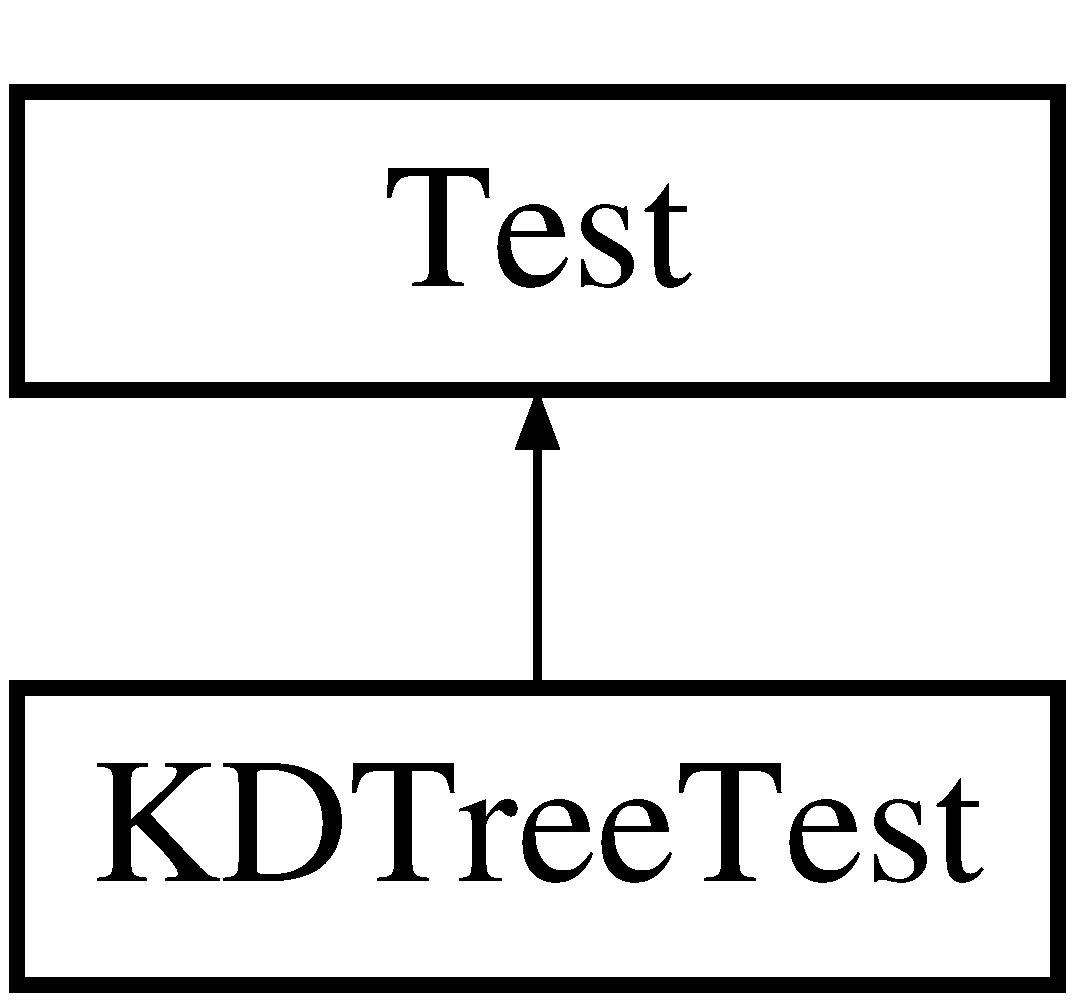
\includegraphics[height=2.000000cm]{classKDTreeTest}
\end{center}
\end{figure}
\subsection*{Static Public Attributes}
\begin{DoxyCompactItemize}
\item 
\hypertarget{classKDTreeTest_a836729a070eb9537d0cc9c960e4e6ebb}{static float $\ast$$\ast$ {\bfseries data}}\label{classKDTreeTest_a836729a070eb9537d0cc9c960e4e6ebb}

\item 
\hypertarget{classKDTreeTest_aeb538469cef4399ec6911856a4c7e407}{static size\-\_\-t {\bfseries N}}\label{classKDTreeTest_aeb538469cef4399ec6911856a4c7e407}

\item 
\hypertarget{classKDTreeTest_ababb08a55d11ed0df1be2befe4bdba49}{static size\-\_\-t {\bfseries d}}\label{classKDTreeTest_ababb08a55d11ed0df1be2befe4bdba49}

\end{DoxyCompactItemize}
\subsection*{Protected Member Functions}
\begin{DoxyCompactItemize}
\item 
\hypertarget{classKDTreeTest_ae64f932fe7a552a1977397f5884e4696}{virtual void {\bfseries Set\-Up} ()}\label{classKDTreeTest_ae64f932fe7a552a1977397f5884e4696}

\item 
\hypertarget{classKDTreeTest_af827d1df2c003a2ae4e755ae2cc83703}{virtual void {\bfseries Tear\-Down} ()}\label{classKDTreeTest_af827d1df2c003a2ae4e755ae2cc83703}

\end{DoxyCompactItemize}
\subsection*{Static Protected Member Functions}
\begin{DoxyCompactItemize}
\item 
\hypertarget{classKDTreeTest_ad769deefe40a92b3865c2ee88a47bd10}{static void {\bfseries Set\-Up\-Test\-Case} ()}\label{classKDTreeTest_ad769deefe40a92b3865c2ee88a47bd10}

\item 
\hypertarget{classKDTreeTest_a3ba954652e64b01aabfc4e2448758d55}{static void {\bfseries Tear\-Down\-Test\-Case} ()}\label{classKDTreeTest_a3ba954652e64b01aabfc4e2448758d55}

\end{DoxyCompactItemize}


\subsection{Detailed Description}
Customized test case for testing 

The documentation for this class was generated from the following file\-:\begin{DoxyCompactItemize}
\item 
/home/hallab/\-Development/\-Tools/workspace/k-\/means/test/test\-\_\-kdtree.\-cpp\end{DoxyCompactItemize}

\hypertarget{structSimpleCluster_1_1KmeansCriteria}{\section{Simple\-Cluster\-:\-:Kmeans\-Criteria Struct Reference}
\label{structSimpleCluster_1_1KmeansCriteria}\index{Simple\-Cluster\-::\-Kmeans\-Criteria@{Simple\-Cluster\-::\-Kmeans\-Criteria}}
}


{\ttfamily \#include $<$k-\/means.\-h$>$}

\subsection*{Public Attributes}
\begin{DoxyCompactItemize}
\item 
\hypertarget{structSimpleCluster_1_1KmeansCriteria_a90eb14d83eaaa78c6aa590cc03db151a}{double {\bfseries alpha}}\label{structSimpleCluster_1_1KmeansCriteria_a90eb14d83eaaa78c6aa590cc03db151a}

\item 
\hypertarget{structSimpleCluster_1_1KmeansCriteria_a417746caabd9c8aa94eae201ebe706ff}{double {\bfseries accuracy}}\label{structSimpleCluster_1_1KmeansCriteria_a417746caabd9c8aa94eae201ebe706ff}

\item 
\hypertarget{structSimpleCluster_1_1KmeansCriteria_a315f994501adf69d674ff6ab57291f91}{int {\bfseries iterations}}\label{structSimpleCluster_1_1KmeansCriteria_a315f994501adf69d674ff6ab57291f91}

\end{DoxyCompactItemize}


\subsection{Detailed Description}
Criteria 

The documentation for this struct was generated from the following file\-:\begin{DoxyCompactItemize}
\item 
/home/hallab/\-Development/\-Tools/workspace/k-\/means/include/k-\/means.\-h\end{DoxyCompactItemize}

\hypertarget{classKmeansTest}{\section{Kmeans\+Test Class Reference}
\label{classKmeansTest}\index{Kmeans\+Test@{Kmeans\+Test}}
}
Inheritance diagram for Kmeans\+Test\+:\begin{figure}[H]
\begin{center}
\leavevmode
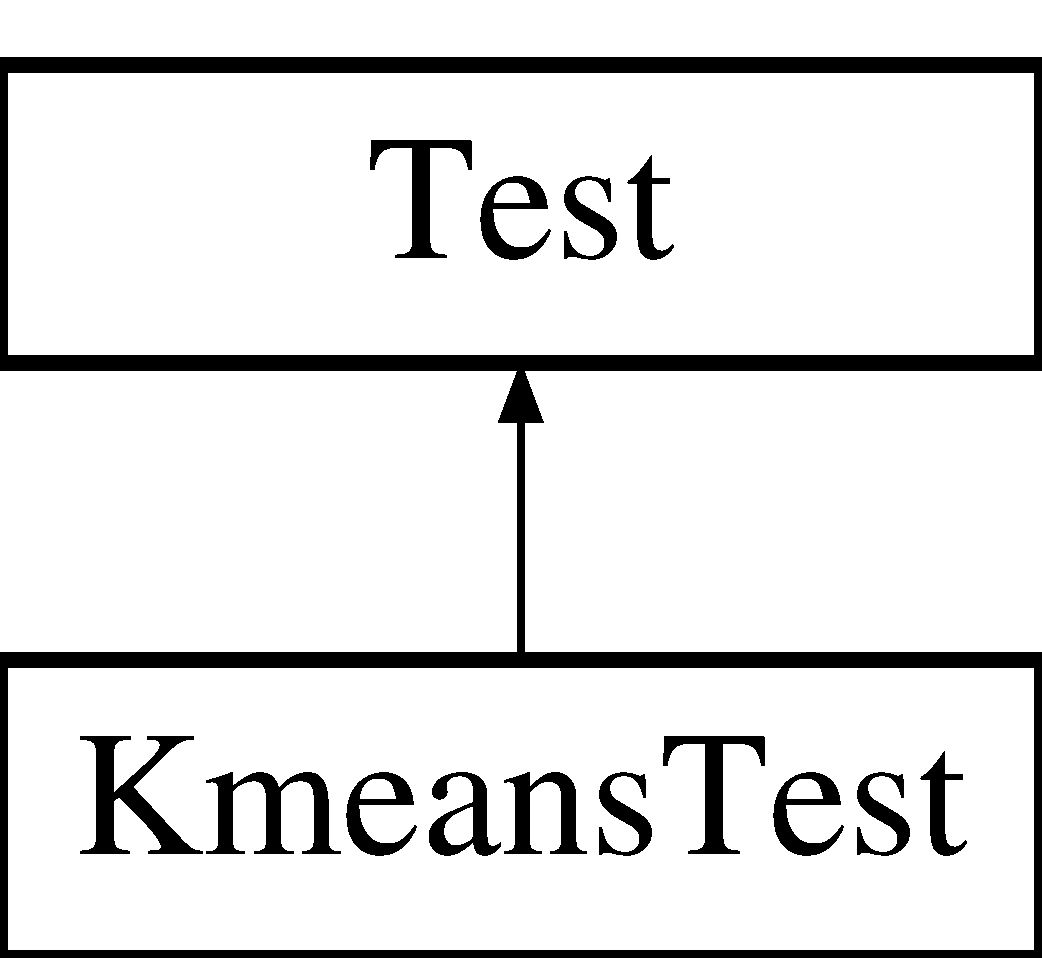
\includegraphics[height=2.000000cm]{classKmeansTest}
\end{center}
\end{figure}
\subsection*{Static Public Attributes}
\begin{DoxyCompactItemize}
\item 
\hypertarget{classKmeansTest_ac49bc85d7f0c6573fdb41291fcad7ea8}{static double $\ast$$\ast$ {\bfseries data}}\label{classKmeansTest_ac49bc85d7f0c6573fdb41291fcad7ea8}

\item 
\hypertarget{classKmeansTest_a02a49c0447e8979c5e42e80798f1909d}{static double $\ast$$\ast$ {\bfseries seeds}}\label{classKmeansTest_a02a49c0447e8979c5e42e80798f1909d}

\item 
\hypertarget{classKmeansTest_ad1d5e54851950f37170c362518fc5aef}{static double $\ast$$\ast$ {\bfseries centroids}}\label{classKmeansTest_ad1d5e54851950f37170c362518fc5aef}

\item 
\hypertarget{classKmeansTest_ab83157ed1cd9481c94b2b5272ca5020d}{static vector$<$ i\+\_\+vector $>$ {\bfseries clusters}}\label{classKmeansTest_ab83157ed1cd9481c94b2b5272ca5020d}

\item 
\hypertarget{classKmeansTest_a881736055281c3d2d5f161a57f37b810}{static int {\bfseries N}}\label{classKmeansTest_a881736055281c3d2d5f161a57f37b810}

\item 
\hypertarget{classKmeansTest_a08d592368c02b1aabe71c26b34796bf6}{static int {\bfseries d}}\label{classKmeansTest_a08d592368c02b1aabe71c26b34796bf6}

\item 
\hypertarget{classKmeansTest_a044e6c5eff9a1a3ddb542771c226bd7b}{static int {\bfseries k}}\label{classKmeansTest_a044e6c5eff9a1a3ddb542771c226bd7b}

\end{DoxyCompactItemize}
\subsection*{Protected Member Functions}
\begin{DoxyCompactItemize}
\item 
\hypertarget{classKmeansTest_a342e848abba368f87b25a0e8c8a511d7}{virtual void {\bfseries Set\+Up} ()}\label{classKmeansTest_a342e848abba368f87b25a0e8c8a511d7}

\item 
\hypertarget{classKmeansTest_a16de3306d32ab3ece3766800ab01fae1}{virtual void {\bfseries Tear\+Down} ()}\label{classKmeansTest_a16de3306d32ab3ece3766800ab01fae1}

\end{DoxyCompactItemize}
\subsection*{Static Protected Member Functions}
\begin{DoxyCompactItemize}
\item 
\hypertarget{classKmeansTest_a5374fc1586536e197b55fd620b3bb2cb}{static void {\bfseries Set\+Up\+Test\+Case} ()}\label{classKmeansTest_a5374fc1586536e197b55fd620b3bb2cb}

\item 
\hypertarget{classKmeansTest_a4e7430b8838dcfbd3f1dab67abd0e466}{static void {\bfseries Tear\+Down\+Test\+Case} ()}\label{classKmeansTest_a4e7430b8838dcfbd3f1dab67abd0e466}

\end{DoxyCompactItemize}


\subsection{Detailed Description}
Customized test case for testing 

The documentation for this class was generated from the following file\+:\begin{DoxyCompactItemize}
\item 
/\+Users/aaa/\+Development/\+Research/simple-\/k-\/means/test/test\+\_\+kmeans.\+cpp\end{DoxyCompactItemize}

\hypertarget{classUtilTest}{\section{Util\+Test Class Reference}
\label{classUtilTest}\index{Util\+Test@{Util\+Test}}
}
Inheritance diagram for Util\+Test\+:\begin{figure}[H]
\begin{center}
\leavevmode
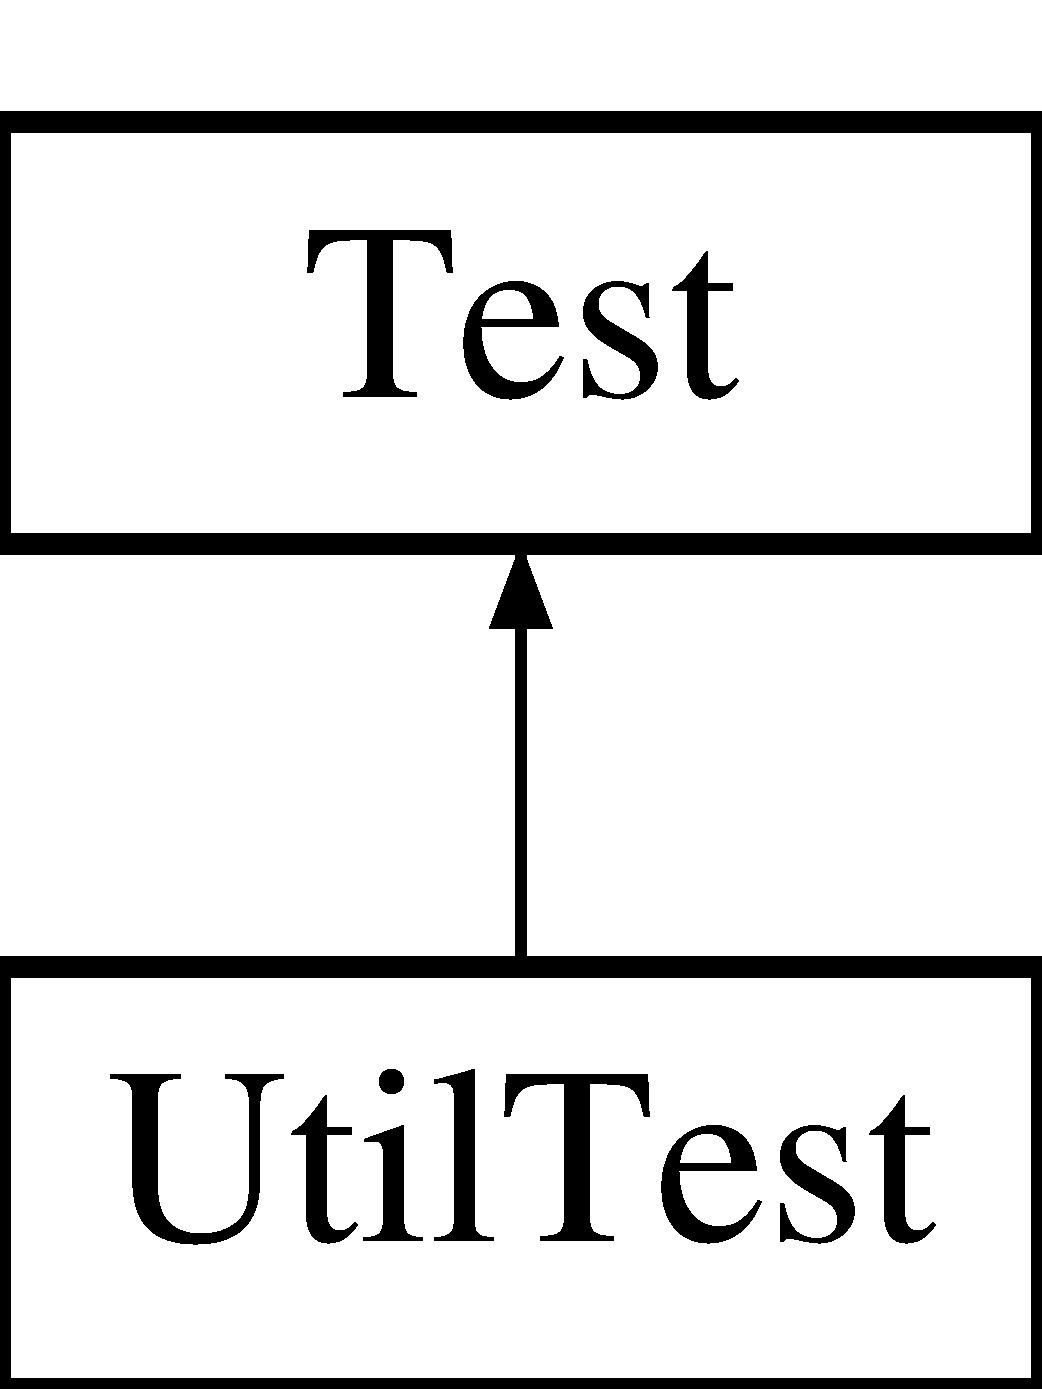
\includegraphics[height=2.000000cm]{classUtilTest}
\end{center}
\end{figure}
\subsection*{Static Public Attributes}
\begin{DoxyCompactItemize}
\item 
\hypertarget{classUtilTest_a13e27888113d6f5f4179c8dd88a39319}{static double $\ast$$\ast$ {\bfseries data}}\label{classUtilTest_a13e27888113d6f5f4179c8dd88a39319}

\item 
\hypertarget{classUtilTest_af0f842c0c1dcc77b49a38a00729bb1b5}{static int {\bfseries N}}\label{classUtilTest_af0f842c0c1dcc77b49a38a00729bb1b5}

\item 
\hypertarget{classUtilTest_a362326a74eb03fd9e035581901c6e103}{static int {\bfseries d}}\label{classUtilTest_a362326a74eb03fd9e035581901c6e103}

\end{DoxyCompactItemize}
\subsection*{Protected Member Functions}
\begin{DoxyCompactItemize}
\item 
\hypertarget{classUtilTest_a8f67bdc9dd37ff9fd862f66ddfb863cb}{virtual void {\bfseries Set\+Up} ()}\label{classUtilTest_a8f67bdc9dd37ff9fd862f66ddfb863cb}

\item 
\hypertarget{classUtilTest_a38fecea095d1c8f8bd55c86292425081}{virtual void {\bfseries Tear\+Down} ()}\label{classUtilTest_a38fecea095d1c8f8bd55c86292425081}

\end{DoxyCompactItemize}
\subsection*{Static Protected Member Functions}
\begin{DoxyCompactItemize}
\item 
\hypertarget{classUtilTest_ac0080980382f83fba5bdf4834196b21d}{static void {\bfseries Set\+Up\+Test\+Case} ()}\label{classUtilTest_ac0080980382f83fba5bdf4834196b21d}

\item 
\hypertarget{classUtilTest_a969e49f758a52c5385f812c55163cc6d}{static void {\bfseries Tear\+Down\+Test\+Case} ()}\label{classUtilTest_a969e49f758a52c5385f812c55163cc6d}

\end{DoxyCompactItemize}


\subsection{Detailed Description}
Customized test case for testing 

The documentation for this class was generated from the following file\+:\begin{DoxyCompactItemize}
\item 
/\+Users/aaa/\+Development/\+Research/simple-\/k-\/means/test/test\+\_\+utilities.\+cpp\end{DoxyCompactItemize}

%--- End generated contents ---

% Index
\newpage
\phantomsection
\addcontentsline{toc}{chapter}{Index}
\printindex

\end{document}
